\documentclass{article}\usepackage[]{graphicx}\usepackage[]{color}
%% maxwidth is the original width if it is less than linewidth
%% otherwise use linewidth (to make sure the graphics do not exceed the margin)
\makeatletter
\def\maxwidth{ %
  \ifdim\Gin@nat@width>\linewidth
    \linewidth
  \else
    \Gin@nat@width
  \fi
}
\makeatother

\definecolor{fgcolor}{rgb}{0.345, 0.345, 0.345}
\newcommand{\hlnum}[1]{\textcolor[rgb]{0.686,0.059,0.569}{#1}}%
\newcommand{\hlstr}[1]{\textcolor[rgb]{0.192,0.494,0.8}{#1}}%
\newcommand{\hlcom}[1]{\textcolor[rgb]{0.678,0.584,0.686}{\textit{#1}}}%
\newcommand{\hlopt}[1]{\textcolor[rgb]{0,0,0}{#1}}%
\newcommand{\hlstd}[1]{\textcolor[rgb]{0.345,0.345,0.345}{#1}}%
\newcommand{\hlkwa}[1]{\textcolor[rgb]{0.161,0.373,0.58}{\textbf{#1}}}%
\newcommand{\hlkwb}[1]{\textcolor[rgb]{0.69,0.353,0.396}{#1}}%
\newcommand{\hlkwc}[1]{\textcolor[rgb]{0.333,0.667,0.333}{#1}}%
\newcommand{\hlkwd}[1]{\textcolor[rgb]{0.737,0.353,0.396}{\textbf{#1}}}%

\usepackage{framed}
\makeatletter
\newenvironment{kframe}{%
 \def\at@end@of@kframe{}%
 \ifinner\ifhmode%
  \def\at@end@of@kframe{\end{minipage}}%
  \begin{minipage}{\columnwidth}%
 \fi\fi%
 \def\FrameCommand##1{\hskip\@totalleftmargin \hskip-\fboxsep
 \colorbox{shadecolor}{##1}\hskip-\fboxsep
     % There is no \\@totalrightmargin, so:
     \hskip-\linewidth \hskip-\@totalleftmargin \hskip\columnwidth}%
 \MakeFramed {\advance\hsize-\width
   \@totalleftmargin\z@ \linewidth\hsize
   \@setminipage}}%
 {\par\unskip\endMakeFramed%
 \at@end@of@kframe}
\makeatother

\definecolor{shadecolor}{rgb}{.97, .97, .97}
\definecolor{messagecolor}{rgb}{0, 0, 0}
\definecolor{warningcolor}{rgb}{1, 0, 1}
\definecolor{errorcolor}{rgb}{1, 0, 0}
\newenvironment{knitrout}{}{} % an empty environment to be redefined in TeX

\usepackage{alltt}
%\usepackage[margin=1in]{geometry}   % set up margins
\usepackage[vmargin=1in,hmargin=1in]{geometry}
\usepackage{tikz}
\usepackage{booktabs}

\usepackage[backend=bibtex]{biblatex}


\thispagestyle{empty}
\begin{center}
\begin{minipage}{1.2\linewidth}
    \centering
 %   \rule{0.4\linewidth}{0.15\linewidth}\par
    \vspace{3cm}
%Thesis title
    \textbf{{\uppercase{\Large German Credit Data Scoring using R\par}}}
    \vspace{2cm}
    %Degree
    {\Large Business and Data Analytics \par}
    {\textit{\hspace{0.5cm}Project Report} \par}
    \vspace{2cm}
    %University logo
   \hspace{1.9cm} 
\includegraphics[width=0.35\linewidth]{hyderabad-university-publishes-mtech.jpg}\newline
    
    {\textit{\hspace{0.5cm}Submitted by} \par}
%Author's name
  \centering
    {\Large Laltendu Das [15MCMI22]\par}
    {\Large Uma Revathi K N [15MCMI20]\par}
    {\Large  Rosni K V [15MCMI15]\par}
    \vspace{1cm}
    
    %Author's name
    {\textit{\hspace{1cm}Under the Guidance of} \par}
    {\Large Dr. V.Ravi, Professor, IDRBT \par}
    \vspace{2cm}
    \centering
%Date
    {\textbf{\Large November 2015}}
\end{minipage}
\end{center}
\clearpage


\newpage
\renewcommand{\contentsname}{\centering Table of Contents}
\newline
\newline
\tableofcontents
\newpage
%\renewcommand{\listfigurename}{\centering List of Figures}
\listoffigures
%\renewcommand{\listoftables}{\centering List of Tables}
\listoftables
\newpage
\IfFileExists{upquote.sty}{\usepackage{upquote}}{}
\begin{document}
%\SweaveOpts{concordance=TRUE}

%\title {An Attractive Template of a Reproducible Data Analysis Document for an Awesome Class Project}
%\author{Mahbubul Majumder, PhD\\ Department of Mathematics\\ University of Nebraska at Omaha }

%\maketitle



\section{Abstract}
\hspace{0.5cm} Credit scoring uses quantitative measures of the performance and characteristics of past loans to predict the future performance of loans with similar characteristics. The objective of credit scoring is to help credit providers quantify and manage the financial risk involved in providing credit so that they can make better lending decisions quickly and more objectively. As a result, various kinds of credit scoring models are established to evaluate the customers' credit rank.
\par A credit scoring system should be able to classify customers as good credit those  who are expected to repay on time and as bad credit those who are expected to fail. A major problem for banks is how to determine the bad credit, because bad credit may cause serious problems in the future. This leads to loss in bank capital, lower bank revenues and subsequently increases bank losses, which can lead to insolvency or bankruptcy. The categorisation of good and bad credit is of fundamental importance, and is indeed the objective of a credit scoring model. Classification models for credit scoring are used to categorize new applicants as either accepted or rejected with respect to these characteristics. In some cases the final selection of the characteristics was based on the statistical analysis used, i.e. logistic regression, neural network etc.
\par This study illustrates the use of data mining techniques to construct credit scoring models. Also, it illustrates the comparison of credit scoring models to give a superior final model. The report also highlights each data mining approach using R language.\\
%\end{abstract}
%\tableofcontents

\section{Introduction} 
\hspace{0.5cm} Credit scoring is one of the applications for predictive modeling, to predict whether or not credit extended to an applicant will likely result in profit or losses for the lending institution. For instance when a bank provides money to an individual, and expects to be paid back in time with interest commensurate with the risk of default. When a bank grants loan to a new customer, bank uses techniques on the large sample of previous customers with their application details and subsequent credit history available. Applying techniques results in connection between the characteristics of the customers.
\par Banks use credit risk modeling in order to measure the amount of credit risk which they are exposed to. The most commonly used technique for this purpose is logistic regression. In our study, we applied different techniques like support vector machines, nearest neighbor, decision trees on data to classify the borrowers as good or bad. So that the borrowers which are classified as bad are not granted any credit.
\par For the experiments, we used the German credit data set which was available in the UCI Repository. The data set consists of 20 attributes (7 numerical and 13 categorical) and there are totally 1000 instances (300 bad and 700 good cases). It was produced by Strathclyde University and is associated with several academic work.
\par In Section 3 we discussed about the risks that are faced by credit scoring model, to grant loan to a new customer. Section 4 consists of dataset that we are used. Section 5 consists of preprocessing steps that are performed on dataset. Statistical analysis is Basic processing of data,including computing statistical quantities, smoothing, testing, and visualizing, gives a first level of analysis. 
\par Under data preprocessing we applied chi-square test, statistical-test and principle component analysis on german credit dataset. Data transformation, in this preprocessing step, the data transformed or consolidated so that the resulting mining process may be more efficient, and the patterns found may be easier to understand. Dealing with categorical data poses some limitations. For example, if data contained too many categories there would be a need to combine several categories into one. Recode a categorical variable with character values into a variable with numeric values is done by \textit{as.numeric} funcion which is available in R.
\par In Section 6, we applied various models on german credit dataset. Our aim is to perform models such as decision tree,support vector machines,logistics regression,k-nearest neighbour and random forest. Analysis of each model on the basis of quality and ROC. We compared each model accuracy and finalised which model is giving better accuracy on given dataset.\\
%The first sentence of this section is so attractive that it made the reader concentrate on reading. The second sentence is so great that it made the reader forget the date. Rest of the sentences are so nice that at the end of the paragraph the reader can't just wait to see what is coming on the next paragraph. At this point reader does not mind if it gets a little technical.  \\
%
%The first sentence of any paragraph presents a clear message. The rest of the sentences just describe that idea and establish the facts so that the reader see the logical conclusion of the paragraph. The last sentence of the paragraph connects the following paragraphs or section.  \\
%
%Add some motivational pictures in this section whenever possible. This will provide the reader some relief from reading text after text. For example Figure \ref{fig:nice-plot} indeed make us happy that we have something else to concentrate. This motivational picture does not need to be generated from the data you are going to analyze. Notice that we added the \textbf{R} codes of generating the Figure~\ref{fig:nice-plot}.
%
%If we don't want to display the R codes, we just put option \texttt{echo=FALSE} in the head of the chunk. To add caption for the figure we write the caption in \texttt{fig.cap=`my figure captions'}.
%
%%%%%%<<nice-plot, fig.cap="My awesome figure caption really describes what this figure is about and what we see in this figure. Also notice that the figure size is kept in such a way that it fits in the text nicely - not too big nor too small", fig.width=4, fig.height=4, fig.align='center',fig.pos="hbtp",out.width='.45\\linewidth'>>=
%plot(women)
%@

%Also please don't forget to explain in details about what this figure is telling. It is really a bad idea not to say anything about the figure when you added it. Its like a product you are selling to someone who don't want to buy it. So, you have to be very serious about selling it with convincing argument.

%\subsection{Preparing this document} 
%This whole document is prepared using \textbf{R}  \cite{R-base} package \texttt{knitr} \cite{R-knitr}. It is a dynamic document and reproducible any number of times for any data sets. To start our work conveniently we need to install \textbf{R}, \texttt{RStudio} and \LaTeX{} \cite{lamport94} . Once our installation is done we will configure \texttt{RStudio} to work with \texttt{knitr}. For this first install \texttt{knitr} using command \texttt{install.packages("knitr")} and include the \texttt{knitr} library by command \texttt{library(knitr)}. Once \texttt{knitr} is installed go to the \texttt{RStudio} menu \texttt{Tools > Global Options...Sweave} and change `Weave Rnw files using' to indicate \texttt{Knitr}.\\

%Now we are ready to create our first document using \texttt{knitr}. Go to \texttt{File > New File > R Sweave} and it will start with a new template for a document. If you save this minimal template it will be saved as a \texttt{.Rnw} file. Now we can just start filling the template with our texts. To create a human readable pdf file from \texttt{.Rnw} we just click on \texttt{Compile PDF} in \texttt{RStudio} toolbar. \\

%{\bf PDF latex failure:} If you encounter any problem such as \texttt{Running pdflatex on ...failed} it could be due to the bibliography. To solve that problem what you can do is: Go back to the folder where you saved your \texttt{.Rnw} file and find the \texttt{.tex} file that is created automatically. Now run the \texttt{.tex} file from \LaTeX{} editor to create the pdf. Once you do this multiple times your bibliographies would be updated and you will be ready to work from \texttt{RStudio} as long as you don't change any object that has references in the file. There may be a better solution for this, but so far this worked for me. \\

%The solution for this problem: just add \texttt{\textbackslash usepackage[backend=bibtex]{biblatex}} in your preamble of the \texttt{.Rnw} file.
\section{Problem definition}\hspace{0.5cm}To develop a credit scoring model to predict the credit risk of applicants as bad risk(default) and good risk, which will help credit providers decide whether to grant loan to customers or not. The associated task for this problem is classification, and the German Credit Data set(source::UCI Machine Learning Repository) \cite{[2]} is using.

\section{About the data} \hspace{0.5cm} To meet with the objective of the analysis, ie, from credit providers perspective, to minimize loss they needs a decision rule regarding who to give approval of the loan and who not to. German Credit Classification dataset obtained from the UCI(University of California,Irvine)Machine Learning Repository \cite{[2]}, was used in this study. The number of examples in this dataset is sufficient and its values for each attribute are complete or available. The detailed description of attributes included in Appendix.\par
The number of examples in the dataset is 1000.The dataset is classified into two classes:good and bad class. The good class has 700 examples whereas the bad one has 300. The dataset has 20 attributes, Seven of the attributes are of continuous(numerical) types, while the other 13 are of categorical types. The summary of data is given below:\\

\begin{knitrout}
\definecolor{shadecolor}{rgb}{0.969, 0.969, 0.969}\color{fgcolor}\begin{kframe}
\begin{alltt}
\hlstd{dataset}\hlkwb{<-}\hlkwd{read.csv}\hlstd{(}\hlstr{"/home/freestyler/BDA_project/Data/german.csv"}\hlstd{)}
\hlkwd{summary}\hlstd{(dataset)}
\end{alltt}
\begin{verbatim}
##  check_status    duration    history      purpose        credit     
##  A11:274      Min.   : 4.0   A30: 40   A43    :280   Min.   :  250  
##  A12:269      1st Qu.:12.0   A31: 49   A40    :234   1st Qu.: 1366  
##  A13: 63      Median :18.0   A32:530   A42    :181   Median : 2320  
##  A14:394      Mean   :20.9   A33: 88   A41    :103   Mean   : 3271  
##               3rd Qu.:24.0   A34:293   A49    : 97   3rd Qu.: 3972  
##               Max.   :72.0             A46    : 50   Max.   :18424  
##                                        (Other): 55                  
##  bonds     jobex          rate       s_status  guarantor    residence    
##  A61:603   A71: 62   Min.   :1.000   A91: 50   A101:907   Min.   :1.000  
##  A62:103   A72:172   1st Qu.:2.000   A92:310   A102: 41   1st Qu.:2.000  
##  A63: 63   A73:339   Median :3.000   A93:548   A103: 52   Median :3.000  
##  A64: 48   A74:174   Mean   :2.973   A94: 92              Mean   :2.845  
##  A65:183   A75:253   3rd Qu.:4.000                        3rd Qu.:4.000  
##                      Max.   :4.000                        Max.   :4.000  
##                                                                          
##  property        age        install     house        nocredit    
##  A121:282   Min.   :19.00   A141:139   A151:179   Min.   :1.000  
##  A122:232   1st Qu.:27.00   A142: 47   A152:713   1st Qu.:1.000  
##  A123:332   Median :33.00   A143:814   A153:108   Median :1.000  
##  A124:154   Mean   :35.55                         Mean   :1.407  
##             3rd Qu.:42.00                         3rd Qu.:2.000  
##             Max.   :75.00                         Max.   :4.000  
##                                                                  
##    job          liable         ph        nri       credibility 
##  A171: 22   Min.   :1.000   A191:596   A201:963   Min.   :1.0  
##  A172:200   1st Qu.:1.000   A192:404   A202: 37   1st Qu.:1.0  
##  A173:630   Median :1.000                         Median :1.0  
##  A174:148   Mean   :1.155                         Mean   :1.3  
##             3rd Qu.:1.000                         3rd Qu.:2.0  
##             Max.   :2.000                         Max.   :2.0  
## 
\end{verbatim}
\end{kframe}
\end{knitrout}

The data may not be tidy and we may have to preprocess the data before our analysis can be done. We will discuss how we prepared the data in the following section.\\

\section{Data Preprocessing} 
%The next step in this study is the statistical analysis of the data.
%You invested lot of times preparing your data for exploration. Why not you describe what you did and how you did. You may add your R codes so that others know what exactly you did. For example let us view the summary of the data as below.
%Try to avoid putting raw output like this in your final report. Instead make a clean table as shown in table \ref{summary-data}. If you have to keep some raw output of your analysis please put them in a section called appendix at the end of the document. If you really believe that you have to put them here, you can do that and thats why we have this example here.
\subsection{Statistical Analysis}
\subsubsection{Chi squared test} Before recoding categorical to numerical data, we performed chi squared statistics in original dataset. Since the number of attributes in this problem is not very high, it is possible to look into the dependency of the response (Credibility) on each of them individually. The test is applied when you have two categorical variables from a single dataset. It is used to determine whether there is a significant association between the two variables. Here we are analysing the relation between each attribute with the target variable. Chi squared test is applied for all categorical variables, Below code snippet shows result for one attribute :

\begin{knitrout}
\definecolor{shadecolor}{rgb}{0.969, 0.969, 0.969}\color{fgcolor}\begin{kframe}
\begin{alltt}
\hlkwd{library}\hlstd{(}\hlstr{"MASS"}\hlstd{)}
\hlstd{data}\hlkwb{<-}\hlkwd{read.csv}\hlstd{(}\hlstr{"/home/freestyler/BDA_project/Data/german.csv"}\hlstd{)}
\hlstd{tbl}\hlkwb{=}\hlkwd{table}\hlstd{(data}\hlopt{$}\hlstd{check_status,data}\hlopt{$}\hlstd{credibility)}
\hlstd{tbl}
\end{alltt}
\begin{verbatim}
##      
##         1   2
##   A11 139 135
##   A12 164 105
##   A13  49  14
##   A14 348  46
\end{verbatim}
\begin{alltt}
\hlkwd{chisq.test}\hlstd{(tbl)}
\end{alltt}
\begin{verbatim}
## 
## 	Pearson's Chi-squared test
## 
## data:  tbl
## X-squared = 123.7209, df = 3, p-value < 2.2e-16
\end{verbatim}
\end{kframe}
\end{knitrout}
\par If the chi square value is large, it tells us that there may be something causing a significant change. A significantly large value will allow us to reject the null hypothesis, which is defined as the prediction that there is no interaction between variables . Basically, if there is a big enough difference between the scores, then we can say something significant happened. If the scores are too close, then we have to conclude that they are basically the same. Overall chi squared result is shown in Table [1].
\begin{table}[t]
\caption{Chi squared statistics}
\centering
\begin{tabular}{c|c|c}
\toprule
Attribute name & Chi square value & p- value \\
\midrule
check\_status & 123.72 & 2.20E-16 \\
history & 61.691 & 1.279e-12 \\
bonds &	36.099	& 0.0000002761\\
purpose	& 33.356	& 0.0001157\\
property	& 23.72	 & 2.86E-05\\
jobex &	18.368	& 0.001045\\
house	 & 18.2 &	0.0001117\\
install &	12.839 &	0.001629\\
s\_status &	9.6052 &	0.02224\\
guarantor	 & 6.6454 &	0.03606\\
nri	& 5.8216	& 0.01583\\
job	 & 1.8852 &	0.5966\\
ph	& 1.1726	& 0.2789\\

\bottomrule
\end{tabular}
\label{tab}
\end{table}

\subsubsection{T-test: statistical test}A t-test is commonly used to determine whether the mean of a population significantly differs from a specific value or from the mean of another population.  If the calculated t value exceeds we say that the means are significantly different at that level of probability. Statistical significance is determined by the size of the difference between the group averages, the sample size, and the standard deviations of the groups. For practical purposes statistical significance suggests that the two larger populations from which we sample are ``actually`` different. The t-value will be positive if the first mean is larger than the second and negative if it is smaller. T test is applied for interval and normal data \cite{[3]} here, Below code snippet shows result for one attribute :
\begin{knitrout}
\definecolor{shadecolor}{rgb}{0.969, 0.969, 0.969}\color{fgcolor}\begin{kframe}
\begin{alltt}
\hlstd{dataset} \hlkwb{<-} \hlkwd{read.csv}\hlstd{(}\hlstr{"/home/freestyler/BDA_project/Data/german_test.csv"}\hlstd{)}
\hlkwd{library}\hlstd{(fBasics,} \hlkwc{quietly}\hlstd{=}\hlnum{TRUE}\hlstd{)}
\hlkwd{locationTest}\hlstd{(}\hlkwd{na.omit}\hlstd{(dataset[dataset[[}\hlstr{"credibility"}\hlstd{]]} \hlopt{==} \hlstr{"1"}\hlstd{,} \hlstr{"duration"}\hlstd{]),}
             \hlkwd{na.omit}\hlstd{(dataset[dataset[[}\hlstr{"credibility"}\hlstd{]]} \hlopt{==} \hlstr{"2"}\hlstd{,} \hlstr{"duration"}\hlstd{]))}
\end{alltt}
\begin{verbatim}
## 
## Title:
##  t Test
## 
## Test Results:
##   PARAMETER:
##     x Observations: 700
##     y Observations: 300
##     mu: 0
##   SAMPLE ESTIMATES:
##     Mean of x: 19.2071
##     Mean of y: 24.86
##     Var  of x: 122.7567
##     Var  of y: 176.4285
##   STATISTIC:
##                 T: -6.4696
##     T | Equal Var: -6.9523
##   P VALUE:
##     Alternative Two-Sided: 2.404e-10 
##     Alternative      Less: 1.202e-10 
##     Alternative   Greater: 1 
##     Alternative Two-Sided | Equal Var: 6.488e-12 
##     Alternative      Less | Equal Var: 3.244e-12 
##     Alternative   Greater | Equal Var: 1 
##   CONFIDENCE INTERVAL:
##     Two-Sided: -7.3697, -3.936
##          Less: -Inf, -4.2129
##       Greater: -7.0928, Inf
##     Two-Sided | Equal Var: -7.2484, -4.0573
##          Less | Equal Var: -Inf, -4.3142
##       Greater | Equal Var: -6.9915, Inf
## 
## Description:
##  Mon Nov  2 19:41:15 2015
\end{verbatim}
\end{kframe}
\end{knitrout}
Once you compute the t-value you have to look it up in a table of significance to test whether the ratio is large enough to say that the difference between the groups is not likely to have been a chance finding. Overall t-test result(for numerical variables) is shown in Table[2] where mean X is the mean of creditworthy group and mean Y is the mean of non creditworthy group, p-value is associated with t-statistics, and it is the probability of rejecting a true null hypothesis or the probability associated with a false positive. Analysing the below table we found that \textit{liable} and \textit{residence} gives less significance. 
\begin{table}[t]
\caption{t test}
\centering
\begin{tabular}{c|c|c|c}
\toprule
Attribute name & Mean X & Mean Y & p- value \\
\midrule
duration & 19.2071 & 24.86 & 2.404e-10 \\
credit & 2985.4571 & 3938.1267 & 0.00002478\\ 
age & 36.2243  & 33.9633  & 0.003788\\
rate & 2.92 & 3.0967 & 0.02034 \\
nocredit & 1.4243 & 1.3667 & 0.1416\\
liable & 1.1557 & 1.1533 & 0.924\\
residence & 2.8429 & 2.85 & 0.925 \\

%TNM\_job	& 103.1401\\
%age &	97.9012\\
%TNM\_s\_status	& 89.2951\\
%TNM\_install	& 89.2527\\
%TNM\_history	& 87.2464\\
%TNM\_jobex	& 75.462\\
%TNM\_house	& 73.4073\\
%rate	& 69.9141\\
%residence	& 67.3383\\
%TNM\_property	& 56.7922\\
%duration	& 53.9899\\
%TNM\_check\_status	& 53.7911\\
%TNM\_ph	& 51.9718\\
%nocredit	& 47.4668\\
%TNM\_nri	& 47.0012\\
%liable	& 46.2794\\
%TNM\_purpose	& 45.281\\
%TNM\_guarantor	& 40.3566\\
%credit	& 36.6441\\
%TNM\_bonds	& 34.6943\\
\bottomrule
\end{tabular}
\label{tab2}
\end{table}

\subsubsection{Principal Component Analysis}Principal Components Analysis can provide insights into the importance of variables in explaining the variation found within a dataset. A principal component is a numeric linear combination of the values of other variables in the dataset that captures maximal variation in the data. The approach to derive principal components is to determine the eigenvalues of the covariance matrix\cite{[5]}. The importants of components can be analysed from rattle shown in below figure[1]. From this we can analyse the cumulative proportion of components and we can include the components into our models based on the threshold value we chose.\\
\begin{figure}[h]
\begin{center}
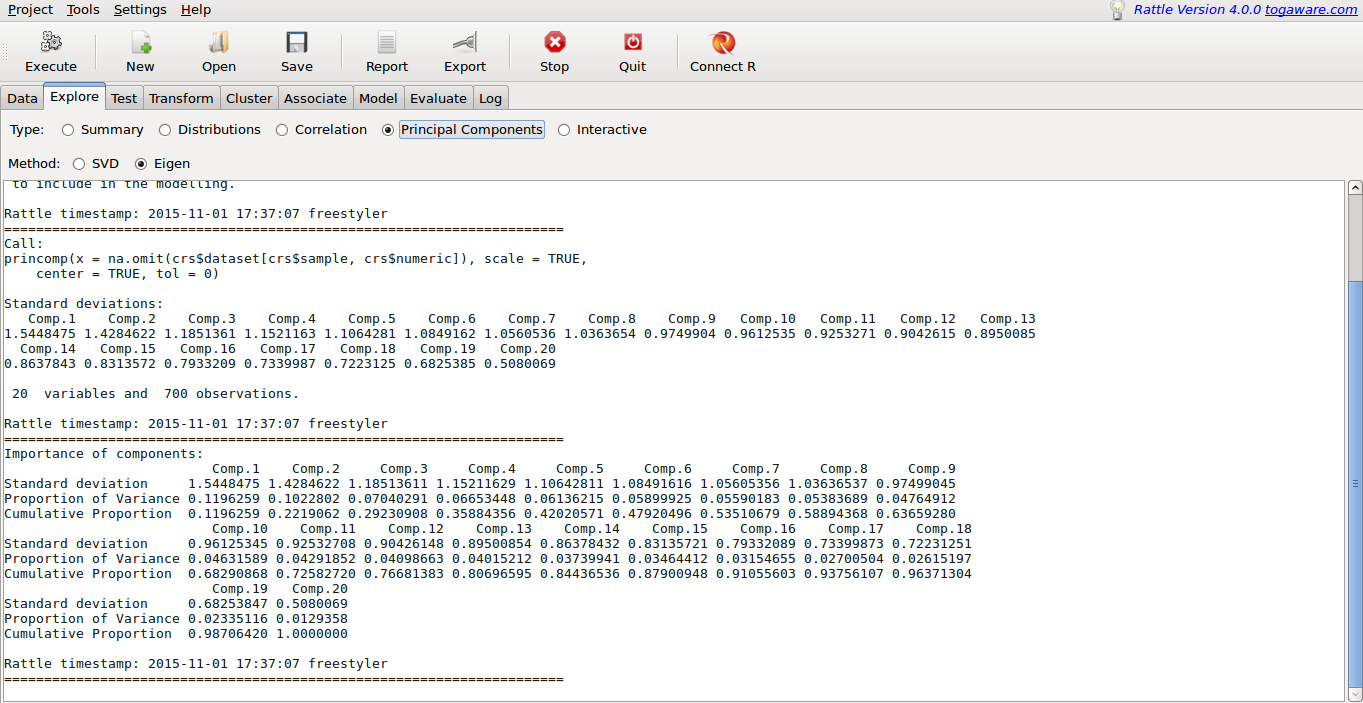
\includegraphics [scale=0.40]{pca.png}
\end{center}
\caption{PCA using eigen value}
\end{figure}

\subsection{Data Transformation}
\subsubsection{Recoding}\hspace{0.5cm}After examine the whole data, it is found that there is no missing values for all attributes. Out of 20 attributes, Seven of the attributes are of continuous(numerical) types, while the other 13 are of categorical types. Using \textit{rattle} package 13 categorical type attributes Recoded as numeric.
\begin{knitrout}
\definecolor{shadecolor}{rgb}{0.969, 0.969, 0.969}\color{fgcolor}\begin{kframe}
\begin{alltt}
\hlstd{dataset} \hlkwb{<-} \hlkwd{read.csv}\hlstd{(}\hlstr{"/home/freestyler/BDA_project/Data/german.csv"}\hlstd{)}
 \hlstd{dataset[[}\hlstr{"TNM_check_status"}\hlstd{]]} \hlkwb{<-} \hlkwd{as.numeric}\hlstd{( dataset[[}\hlstr{"check_status"}\hlstd{]])}
 \hlstd{dataset[[}\hlstr{"TNM_history"}\hlstd{]]} \hlkwb{<-} \hlkwd{as.numeric}\hlstd{( dataset[[}\hlstr{"history"}\hlstd{]])}
 \hlstd{dataset[[}\hlstr{"TNM_purpose"}\hlstd{]]} \hlkwb{<-} \hlkwd{as.numeric}\hlstd{( dataset[[}\hlstr{"purpose"}\hlstd{]])}
 \hlstd{dataset[[}\hlstr{"TNM_bonds"}\hlstd{]]} \hlkwb{<-} \hlkwd{as.numeric}\hlstd{( dataset[[}\hlstr{"bonds"}\hlstd{]])}
 \hlstd{dataset[[}\hlstr{"TNM_jobex"}\hlstd{]]} \hlkwb{<-} \hlkwd{as.numeric}\hlstd{( dataset[[}\hlstr{"jobex"}\hlstd{]])}
 \hlstd{dataset[[}\hlstr{"TNM_s_status"}\hlstd{]]} \hlkwb{<-} \hlkwd{as.numeric}\hlstd{( dataset[[}\hlstr{"s_status"}\hlstd{]])}
 \hlstd{dataset[[}\hlstr{"TNM_guarantor"}\hlstd{]]} \hlkwb{<-} \hlkwd{as.numeric}\hlstd{( dataset[[}\hlstr{"guarantor"}\hlstd{]])}
 \hlstd{dataset[[}\hlstr{"TNM_property"}\hlstd{]]} \hlkwb{<-} \hlkwd{as.numeric}\hlstd{( dataset[[}\hlstr{"property"}\hlstd{]])}
 \hlstd{dataset[[}\hlstr{"TNM_install"}\hlstd{]]} \hlkwb{<-} \hlkwd{as.numeric}\hlstd{( dataset[[}\hlstr{"install"}\hlstd{]])}
 \hlstd{dataset[[}\hlstr{"TNM_house"}\hlstd{]]} \hlkwb{<-} \hlkwd{as.numeric}\hlstd{( dataset[[}\hlstr{"house"}\hlstd{]])}
 \hlstd{dataset[[}\hlstr{"TNM_job"}\hlstd{]]} \hlkwb{<-} \hlkwd{as.numeric}\hlstd{( dataset[[}\hlstr{"job"}\hlstd{]])}
 \hlstd{dataset[[}\hlstr{"TNM_ph"}\hlstd{]]} \hlkwb{<-} \hlkwd{as.numeric}\hlstd{( dataset[[}\hlstr{"ph"}\hlstd{]])}
 \hlstd{dataset[[}\hlstr{"TNM_nri"}\hlstd{]]} \hlkwb{<-} \hlkwd{as.numeric}\hlstd{( dataset[[}\hlstr{"nri"}\hlstd{]])}
\end{alltt}
\end{kframe}
\end{knitrout}
\subsubsection{Rescaling}\hspace{0.5cm}Using \textit{reshape} library the outcome values (1 = Good, 2 = Bad) rescaled to (0 = Good, 1 = Bad).\par
\begin{knitrout}
\definecolor{shadecolor}{rgb}{0.969, 0.969, 0.969}\color{fgcolor}\begin{kframe}
\begin{alltt}
\hlkwd{library}\hlstd{(reshape,} \hlkwc{quietly}\hlstd{=}\hlnum{TRUE}\hlstd{)}
\hlstd{dataset[[}\hlstr{"R01_credibility"}\hlstd{]]} \hlkwb{<-} \hlstd{dataset[[}\hlstr{"credibility"}\hlstd{]]}
\hlstd{dataset[[}\hlstr{"R01_credibility"}\hlstd{]]} \hlkwb{<-} \hlstd{( dataset[[}\hlstr{"credibility"}\hlstd{]]} \hlopt{-} \hlnum{1.000000}\hlstd{)}\hlopt{/}\hlkwd{abs}\hlstd{(}\hlnum{2.000000} \hlopt{-} \hlnum{1.000000}\hlstd{)}
\end{alltt}
\end{kframe}
\end{knitrout}
\subsubsection{Over sampling}\hspace{0.5cm}As we know that the dataset is classified into two classes:good and bad class. The good class has 700 examples whereas the bad one has 300.  Learning from data sets that contain very few instances of the minority (or interesting) class usually produces biased classifiers that have a higher predictive accuracy over the majority class(es), but poorer predictive accuracy over the minority class. \par
\begin{knitrout}
\definecolor{shadecolor}{rgb}{0.969, 0.969, 0.969}\color{fgcolor}\begin{kframe}
\begin{alltt}
\hlstd{dataset}\hlkwb{<-}\hlkwd{read.csv}\hlstd{(}\hlstr{"/home/freestyler/BDA_project/Data/outfile.csv"}\hlstd{)}
\hlstd{df}\hlkwb{<-} \hlkwd{data.frame}\hlstd{(dataset)}
\hlkwd{table}\hlstd{(df}\hlopt{$}\hlstd{R01_credibility)}
\end{alltt}
\begin{verbatim}
## 
##   0   1 
## 700 300
\end{verbatim}
\end{kframe}
\end{knitrout}
\hspace{0.5cm}Using the \textit{unbalanced} package available for R, which implements some of most well-known techniques and propose a racing algorithm to select adaptively the most appropriate strategy for a given unbalanced task. Here we are using \textit{ubOver} \cite{[1]} function for oversampling, the function replicates randomly some instances from the minority class in order to obtain a final dataset with the same number of instances from the two classes.\par


\begin{knitrout}
\definecolor{shadecolor}{rgb}{0.969, 0.969, 0.969}\color{fgcolor}\begin{kframe}
\begin{alltt}
\hlkwd{library}\hlstd{(unbalanced)}
\hlstd{n} \hlkwb{<-}\hlkwd{ncol}\hlstd{(train)}
\hlstd{out} \hlkwb{<-} \hlstd{ytrain}
\hlstd{input} \hlkwb{<-} \hlstd{xtrain}

\hlkwd{table}\hlstd{(ytrain)}
\end{alltt}
\begin{verbatim}
## ytrain
##   0   1 
## 485 215
\end{verbatim}
\begin{alltt}
\hlstd{outdata}\hlkwb{<-} \hlkwd{ubOver}\hlstd{(}\hlkwc{X}\hlstd{=input,} \hlkwc{Y}\hlstd{= out)}
\end{alltt}
\end{kframe}
\end{knitrout}



\begin{knitrout}
\definecolor{shadecolor}{rgb}{0.969, 0.969, 0.969}\color{fgcolor}\begin{kframe}
\begin{alltt}
\hlstd{train_dataset}\hlkwb{<-}\hlkwd{read.csv}\hlstd{(}\hlstr{"/home/freestyler/BDA_project/Data/overSampled_data.csv"}\hlstd{)}
\hlstd{df}\hlkwb{<-} \hlkwd{data.frame}\hlstd{(train_dataset)}
\hlkwd{table}\hlstd{(train_dataset}\hlopt{$}\hlstd{R01_credibility)}
\end{alltt}
\begin{verbatim}
## 
##   0   1 
## 485 485
\end{verbatim}
\end{kframe}
\end{knitrout}

\par\hspace{0.5cm}By analysing the result from above methods, two attributes has been deleted. We assume that the attributes \textit{liable} and \textit{residence} are less significant to contribute for loan sanction. 
%\subsection{What is funny} This section may not be necessary. But if you notice something  about the data that does not make any sense you can mention them in a section like that. Or if you think of anything interesting about the data, just discuss them here.

\section{Methodology} This section will include the methods we used for our analysis. The techniques we studied for this classification problem are Logistic Regression, Decision Tree, Support Vector Machine, Neural network, Random forest  available with \textit{rattle} package.  Other than that we experimented k nearest neighbour and PCA- Neural network .
%You should include some theoretical justification here. For example, why you think the method is applicable, what are the assumptions about the methods, whether your data satisfies those assumption or not etc. 

\subsection{Logistic Regression} \hspace{0.9cm}Logistic regression models are quite useful for classifying new cases into one of two outcome categories (``success" or ``failure"). The estimated logistic model, applied to new cases of a test (evaluation) data set, provides predictions of success probabilities. With a certain cutoff on the predicted success probabilities, the logistic regression provides a rule for classifying new cases. One can use the actual realizations of the cases in the test (evaluation) data set to investigate whether the logistic regression (or any other classification method) is in fact capable of identifying the
actual outcomes. 
\par \hspace{0.5}The logistic regression model links the predictor variables to probabilities
through the equation:

\begin{equation} \label{eq:reg}
 p = f(\alpha + \beta_1 X_1 + \beta_2 X_2 + ....+ \beta_k X_k ) = \frac{exp(\alpha + \beta_1 X_1 + \beta_2 X_2 + ....+ \beta_k X_k )}{1+exp(\alpha + \beta_1 X_1 + \beta_2 X_2 + ....+ \beta_k X_k ) }
\end{equation}
% It can be verified that this function leads to S- shaped curves between 0 and 1 such as those shown in the  graph :
 
% \begin{figure}[h]
%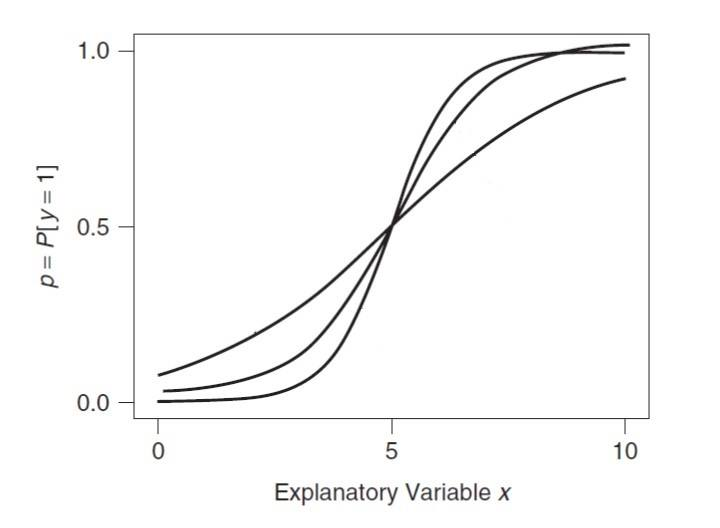
\includegraphics [scale=0.5]{image1.jpg}
%\caption{S  curve}
%\end{figure}

We randomly select 800 of the 1000 cases for the training set, and put the remaining 200 cases to the test set .The R program and its output for the model is listed below.

\begin{knitrout}
\definecolor{shadecolor}{rgb}{0.969, 0.969, 0.969}\color{fgcolor}\begin{kframe}
\begin{alltt}
\hlkwd{library}\hlstd{(rattle)}
\hlstd{dataset}\hlkwb{<-}\hlkwd{read.csv}\hlstd{(}\hlstr{"/home/freestyler/BDA_project/Data/outfile.csv"}\hlstd{)}
\hlkwd{set.seed}\hlstd{(}\hlnum{42}\hlstd{)}
\hlstd{nobs} \hlkwb{<-} \hlkwd{nrow}\hlstd{(dataset)} \hlcom{# 1000 observations }
\hlstd{sample} \hlkwb{<-} \hlstd{train} \hlkwb{<-} \hlkwd{sample}\hlstd{(}\hlkwd{nrow}\hlstd{(dataset),} \hlnum{0.8}\hlopt{*}\hlstd{nobs)} \hlcom{# 800 observations}
\hlstd{validate} \hlkwb{<-} \hlkwa{NULL}
\hlstd{test} \hlkwb{<-} \hlkwd{setdiff}\hlstd{(}\hlkwd{setdiff}\hlstd{(}\hlkwd{seq_len}\hlstd{(}\hlkwd{nrow}\hlstd{(dataset)), train), validate)} \hlcom{# 200 observations}
\end{alltt}
\end{kframe}
\end{knitrout}


\\ The regression model built. The code below estimates a logistic regression model using the glm (generalized linear model) function.
\begin{knitrout}
\definecolor{shadecolor}{rgb}{0.969, 0.969, 0.969}\color{fgcolor}\begin{kframe}
\begin{alltt}
\hlstd{glm} \hlkwb{<-} \hlkwd{glm}\hlstd{(R01_credibility} \hlopt{~} \hlstd{.,}
               \hlkwc{data}\hlstd{=dataset[train,} \hlkwd{c}\hlstd{(input, target)],}
               \hlkwc{family}\hlstd{=}\hlkwd{binomial}\hlstd{(}\hlkwc{link}\hlstd{=}\hlstr{"logit"}\hlstd{))}

\hlkwd{print}\hlstd{(}\hlkwd{summary}\hlstd{(glm))}
\end{alltt}
\begin{verbatim}
## 
## Call:
## glm(formula = R01_credibility ~ ., family = binomial(link = "logit"), 
##     data = dataset[train, c(input, target)])
## 
## Deviance Residuals: 
##     Min       1Q   Median       3Q      Max  
## -1.9202  -0.7486  -0.4362   0.7863   2.4630  
## 
## Coefficients:
##                    Estimate Std. Error z value Pr(>|z|)    
## (Intercept)       5.373e+00  1.124e+00   4.780 1.76e-06 ***
## duration          2.853e-02  9.914e-03   2.878 0.004000 ** 
## credit            5.210e-05  4.466e-05   1.167 0.243310    
## rate              2.451e-01  9.297e-02   2.636 0.008390 ** 
## age              -1.037e-02  8.889e-03  -1.166 0.243500    
## nocredit          2.765e-01  1.760e-01   1.571 0.116141    
## TNM_check_status -5.992e-01  7.818e-02  -7.664 1.80e-14 ***
## TNM_history      -4.278e-01  9.663e-02  -4.427 9.55e-06 ***
## TNM_purpose      -3.784e-02  3.433e-02  -1.102 0.270388    
## TNM_bonds        -2.234e-01  6.714e-02  -3.327 0.000877 ***
## TNM_jobex        -1.637e-01  7.835e-02  -2.089 0.036686 *  
## TNM_s_status     -1.996e-01  1.251e-01  -1.595 0.110604    
## TNM_guarantor    -5.074e-01  2.016e-01  -2.516 0.011866 *  
## TNM_property      1.817e-01  1.000e-01   1.817 0.069292 .  
## TNM_install      -3.320e-01  1.270e-01  -2.614 0.008955 ** 
## TNM_house        -2.212e-01  1.847e-01  -1.198 0.230959    
## TNM_job          -9.282e-02  1.505e-01  -0.617 0.537296    
## TNM_ph           -2.969e-01  2.085e-01  -1.424 0.154394    
## TNM_nri          -1.044e+00  6.230e-01  -1.676 0.093835 .  
## ---
## Signif. codes:  0 '***' 0.001 '**' 0.01 '*' 0.05 '.' 0.1 ' ' 1
## 
## (Dispersion parameter for binomial family taken to be 1)
## 
##     Null deviance: 985.71  on 799  degrees of freedom
## Residual deviance: 766.61  on 781  degrees of freedom
## AIC: 804.61
## 
## Number of Fisher Scoring iterations: 5
\end{verbatim}
\end{kframe}
\end{knitrout}
\\ When developing models for prediction, the most critical metric regards how well the model does in predicting the target variable on out of sample observations. This process involves using the model estimates to predict values on the test set. Afterwards, we compared the predicted target variable versus the observed values for each observation.
\begin{knitrout}
\definecolor{shadecolor}{rgb}{0.969, 0.969, 0.969}\color{fgcolor}\begin{kframe}
\begin{alltt}
\hlkwd{library}\hlstd{(ROCR)}
\hlkwd{library}\hlstd{(ggplot2,} \hlkwc{quietly}\hlstd{=}\hlnum{TRUE}\hlstd{)}

\hlstd{pr} \hlkwb{<-} \hlkwd{predict}\hlstd{(glm,} \hlkwc{type}\hlstd{=}\hlstr{"response"}\hlstd{,} \hlkwc{newdata}\hlstd{=dataset[test,} \hlkwd{c}\hlstd{(input, target)])}
\end{alltt}
\end{kframe}
\end{knitrout}




The ROC curve is plotted Figure [2] and the Area Under Curve obtained is 0.8.\\
\begin{knitrout}
\definecolor{shadecolor}{rgb}{0.969, 0.969, 0.969}\color{fgcolor}\begin{kframe}
\begin{alltt}
\hlkwd{plot}\hlstd{(p)}
\end{alltt}
\end{kframe}\begin{figure}
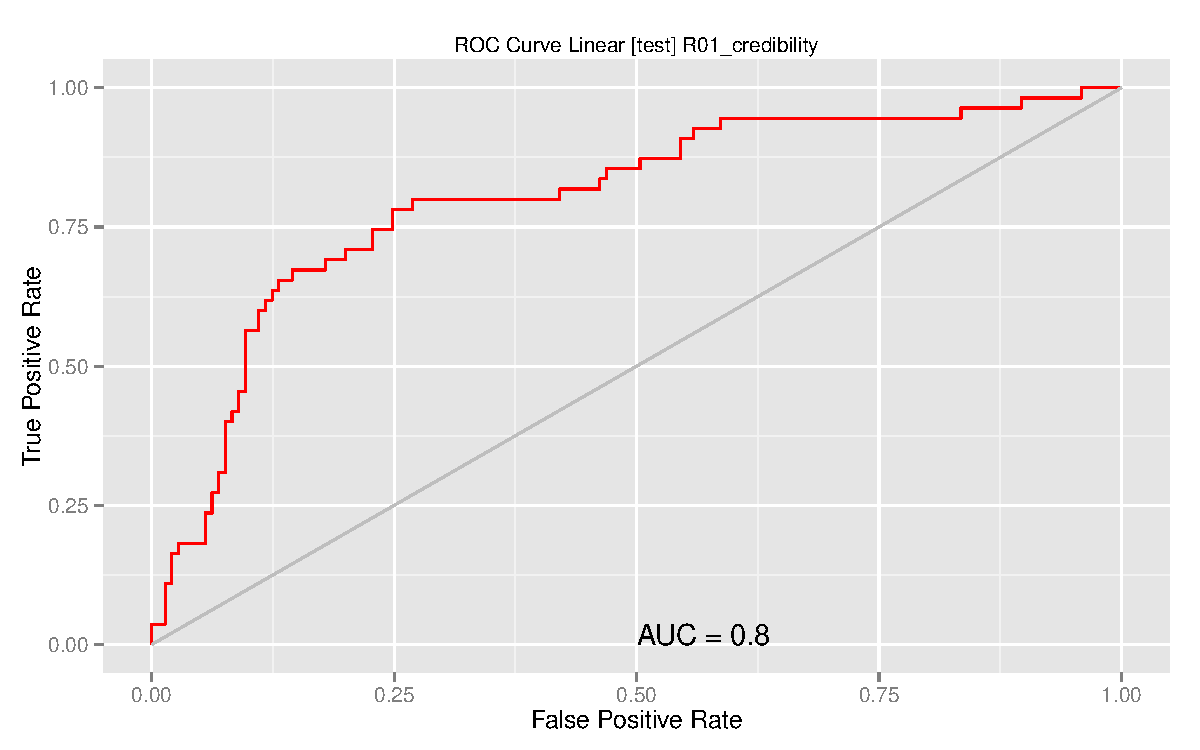
\includegraphics[width=\maxwidth]{figure/unnamed-chunk-18-1} \caption[ROC Curve-Logistic Regression]{ROC Curve-Logistic Regression}\label{fig:unnamed-chunk-18}
\end{figure}


\end{knitrout}
%\begin{figure}[h]
%\begin{center}
%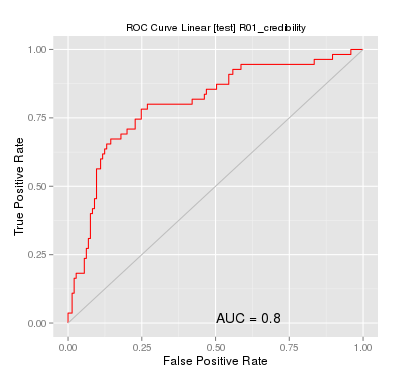
\includegraphics [scale=0.75]{Rplot.png}
%\end{center}
%\caption{ROC Curve:Logistic Regression}
%\end{figure}
\hspace{0cm}The error matrix for the model generated. Below code produce the confusion(error) matrix showing counts.
\begin{knitrout}
\definecolor{shadecolor}{rgb}{0.969, 0.969, 0.969}\color{fgcolor}\begin{kframe}
\begin{alltt}
\hlstd{pr} \hlkwb{<-} \hlkwd{as.vector}\hlstd{(}\hlkwd{ifelse}\hlstd{(}\hlkwd{predict}\hlstd{(glm,} \hlkwc{type}\hlstd{=}\hlstr{"response"}\hlstd{,}
                               \hlkwc{newdata}\hlstd{=dataset[test,} \hlkwd{c}\hlstd{(input, target)])} \hlopt{>} \hlnum{0.5}\hlstd{,} \hlstr{"1"}\hlstd{,} \hlstr{"0"}\hlstd{))}

\hlkwd{table}\hlstd{(dataset[test,} \hlkwd{c}\hlstd{(input, target)]}\hlopt{$}\hlstd{R01_credibility, pr,}
      \hlkwc{dnn}\hlstd{=}\hlkwd{c}\hlstd{(}\hlstr{"Actual"}\hlstd{,} \hlstr{"Predicted"}\hlstd{))}
\end{alltt}
\begin{verbatim}
##       Predicted
## Actual   0   1
##      0 131  14
##      1  27  28
\end{verbatim}
\end{kframe}
\end{knitrout}


\hspace{0cm}And the overall error percentage is :\par
\begin{knitrout}
\definecolor{shadecolor}{rgb}{0.969, 0.969, 0.969}\color{fgcolor}\begin{kframe}
\begin{alltt}
\hlkwd{overall}\hlstd{(}\hlkwd{table}\hlstd{(pr, dataset[test,} \hlkwd{c}\hlstd{(input, target)]}\hlopt{$}\hlstd{R01_credibility,}
              \hlkwc{dnn}\hlstd{=}\hlkwd{c}\hlstd{(}\hlstr{"Predicted"}\hlstd{,} \hlstr{"Actual"}\hlstd{)))}
\end{alltt}
\begin{verbatim}
## 0.205
\end{verbatim}
\end{kframe}
\end{knitrout}


The error matrix showing the proportion is :
\begin{knitrout}
\definecolor{shadecolor}{rgb}{0.969, 0.969, 0.969}\color{fgcolor}\begin{kframe}
\begin{alltt}
\hlstd{per} \hlkwb{<-} \hlkwd{pcme}\hlstd{(dataset[test,} \hlkwd{c}\hlstd{(input, target)]}\hlopt{$}\hlstd{R01_credibility, pr)}
\hlkwd{round}\hlstd{(per,} \hlnum{2}\hlstd{)}
\end{alltt}
\begin{verbatim}
##       Predicted
## Actual    0    1 Error
##      0 0.66 0.07  0.10
##      1 0.14 0.14  0.49
\end{verbatim}
\end{kframe}
\end{knitrout}
From above error matrix we will get sensitivity and specificity proportion as (1-error) from first row and second row respectively. The plot in Figure [2] gives sensitivity(true positive rate) against specificity(true negative rate) :


\begin{knitrout}
\definecolor{shadecolor}{rgb}{0.969, 0.969, 0.969}\color{fgcolor}\begin{kframe}
\begin{alltt}
\hlkwd{plot}\hlstd{(}\hlkwd{performance}\hlstd{(pred,} \hlstr{"sens"}\hlstd{,} \hlstr{"spec"}\hlstd{),} \hlkwc{col}\hlstd{=}\hlstr{"#CC0000FF"}\hlstd{,} \hlkwc{lty}\hlstd{=}\hlnum{1}\hlstd{,} \hlkwc{add}\hlstd{=}\hlnum{FALSE}\hlstd{)}
\end{alltt}
\end{kframe}\begin{figure}
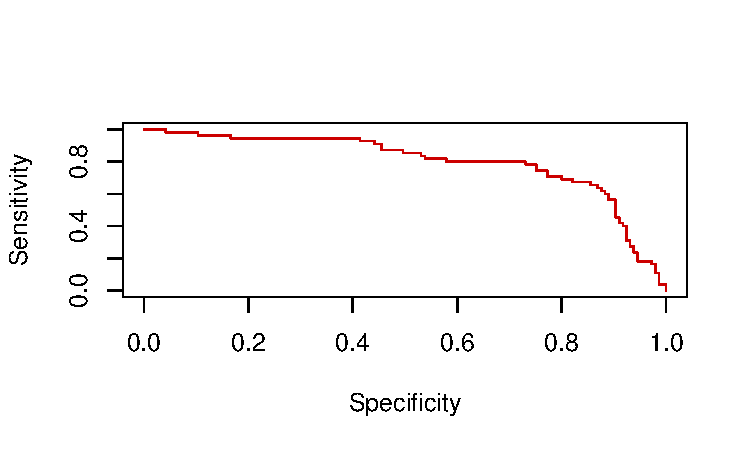
\includegraphics[width=\maxwidth]{figure/unnamed-chunk-25-1} \caption[Sensitivity/Specificity-Logistic Regression]{Sensitivity/Specificity-Logistic Regression}\label{fig:unnamed-chunk-25}
\end{figure}


\end{knitrout}
%\begin{figure}[h]
%\begin{center}
%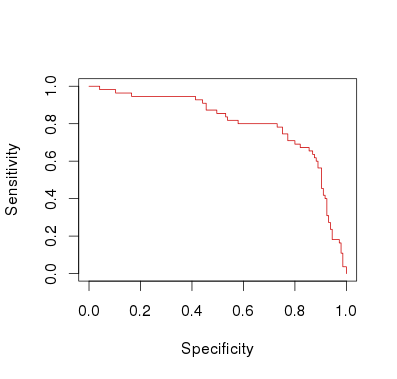
\includegraphics [scale=0.60]{Rplot01.png}
%\end{center}
%\caption{sensitivity/specificity plot:Logistic Regression}
%\end{figure}

Thus the whole performance of Logistic Regression model is analysed by the measures discussed above, and it is giving an accuracy of 79.5\%.\par
%%%%%%%%%%%%%%%%%%%%%%%%%%%%%%%%%%%%%%%%%%%%%%
The k-fold cross validation method involves splitting the dataset into k-subsets. For each subset is held out while the model is trained on all other subsets. This process is completed until accuracy is determine for each instance in the dataset, and an overall accuracy estimate is provided. We observe that we have the same number of examples in each fold. We applied 10-fold cross validation on 1000 samples of the german credit dataset using the package \textit{survival}.
\begin{knitrout}
\definecolor{shadecolor}{rgb}{0.969, 0.969, 0.969}\color{fgcolor}\begin{kframe}
\begin{alltt}
\hlkwd{library}\hlstd{(survival)}
\hlstd{dataset} \hlkwb{<-} \hlkwd{read.csv}\hlstd{(}\hlstr{"/home/freestyler/BDA_project/Data/outfile.csv"}\hlstd{)}
\hlstd{n}\hlkwb{<-}\hlkwd{nrow}\hlstd{(dataset)}
\hlstd{K}\hlkwb{<-}\hlnum{10}
\hlstd{divide}\hlkwb{<-} \hlstd{n} \hlopt \hlstd{K}
\hlkwd{set.seed}\hlstd{(}\hlnum{5}\hlstd{)}
\hlstd{unirand}\hlkwb{<-}\hlkwd{runif}\hlstd{(n)}
\hlstd{rang}\hlkwb{<-}\hlkwd{rank}\hlstd{(unirand)}
\hlstd{bloc}\hlkwb{<-}\hlstd{(rang} \hlopt{-} \hlnum{1}\hlstd{)}\hlopt\hlstd{divide} \hlopt{+}\hlnum{1}
\hlstd{bloc}\hlkwb{<-}\hlkwd{as.factor}\hlstd{(bloc)}
\hlkwd{print}\hlstd{(}\hlkwd{summary}\hlstd{(bloc))}
\end{alltt}
\begin{verbatim}
##   1   2   3   4   5   6   7   8   9  10 
## 100 100 100 100 100 100 100 100 100 100
\end{verbatim}
\end{kframe}
\end{knitrout}
We can repeat now the learning process and the test process. We collect each value in a vector. Printing each sub-sample's sensitivity ,specificity and accuracy :
\begin{knitrout}
\definecolor{shadecolor}{rgb}{0.969, 0.969, 0.969}\color{fgcolor}\begin{kframe}
\begin{alltt}
\hlstd{all.sense}\hlkwb{<-}\hlkwd{numeric}\hlstd{(}\hlnum{0}\hlstd{)}
\hlstd{all.spese}\hlkwb{<-}\hlkwd{numeric}\hlstd{(}\hlnum{0}\hlstd{)}
\hlstd{all.acc1}\hlkwb{<-}\hlkwd{numeric}\hlstd{(}\hlnum{0}\hlstd{)}
\hlkwa{for}\hlstd{(k} \hlkwa{in} \hlnum{1}\hlopt{:}\hlstd{K)\{}
\hlstd{glm} \hlkwb{<-} \hlkwd{glm}\hlstd{(R01_credibility} \hlopt{~}\hlstd{.,} \hlkwc{data} \hlstd{= dataset[bloc}\hlopt{!=}\hlstd{k,],} \hlkwc{family}\hlstd{=}\hlkwd{binomial}\hlstd{(}\hlkwc{link}\hlstd{=}\hlstr{"logit"}\hlstd{))}
\hlstd{pred} \hlkwb{<-} \hlkwd{as.vector}\hlstd{(}\hlkwd{ifelse}\hlstd{(}\hlkwd{predict}\hlstd{(glm,}\hlkwc{newdata} \hlstd{= dataset[bloc}\hlopt{==}\hlstd{k,],}\hlkwc{type} \hlstd{=} \hlstr{'response'}\hlstd{)}
                         \hlopt{>} \hlnum{0.5}\hlstd{,} \hlstr{"1"}\hlstd{,} \hlstr{"0"}\hlstd{))}
\hlcom{#confusion matrix for each partition}
\hlstd{mc}\hlkwb{<-}\hlkwd{table}\hlstd{(dataset}\hlopt{$}\hlstd{R01_credibility[bloc}\hlopt{==}\hlstd{k],pred)}
\hlstd{err}\hlkwb{<-}\hlnum{1.0} \hlopt{-} \hlstd{(mc[}\hlnum{1}\hlstd{,}\hlnum{1}\hlstd{]}\hlopt{+}\hlstd{mc[}\hlnum{2}\hlstd{,}\hlnum{2}\hlstd{])}\hlopt{/}\hlkwd{sum}\hlstd{(mc)}
\hlstd{acc1}\hlkwb{<-}\hlnum{1}\hlopt{-}\hlstd{(err)}
\hlstd{a}\hlkwb{<-}\hlstd{mc[}\hlnum{1}\hlstd{,}\hlnum{1}\hlstd{]}
\hlstd{b}\hlkwb{<-}\hlstd{mc[}\hlnum{1}\hlstd{,}\hlnum{1}\hlstd{]}\hlopt{+}\hlstd{mc[}\hlnum{1}\hlstd{,}\hlnum{2}\hlstd{]}
\hlstd{sensitivity}\hlkwb{<-}\hlstd{a}\hlopt{/}\hlstd{b}
\hlstd{c}\hlkwb{<-}\hlstd{mc[}\hlnum{2}\hlstd{,}\hlnum{2}\hlstd{]}
\hlstd{d}\hlkwb{<-}\hlstd{mc[}\hlnum{2}\hlstd{,}\hlnum{2}\hlstd{]}\hlopt{+}\hlstd{mc[}\hlnum{2}\hlstd{,}\hlnum{1}\hlstd{]}
\hlstd{specificity}\hlkwb{<-}\hlstd{c}\hlopt{/}\hlstd{d}
\hlcom{#function combines vector, matrix or data frame by rows.}
\hlstd{all.sense}\hlkwb{<-}\hlkwd{rbind}\hlstd{(all.sense,sensitivity)}
\hlstd{all.spese}\hlkwb{<-}\hlkwd{rbind}\hlstd{(all.spese,specificity)}
\hlcom{#all.err <- rbind(all.err,err)}
\hlstd{all.acc1}\hlkwb{<-}\hlkwd{rbind}\hlstd{(all.acc1,acc1)}
\hlstd{\}}
\end{alltt}
\end{kframe}
\end{knitrout}
The sensitivity, specificity and accuracy in each fold is listed below
\begin{knitrout}
\definecolor{shadecolor}{rgb}{0.969, 0.969, 0.969}\color{fgcolor}\begin{kframe}
\begin{alltt}
\hlkwd{print}\hlstd{(all.sense)}
\end{alltt}
\begin{verbatim}
##                  [,1]
## sensitivity 0.8750000
## sensitivity 0.9253731
## sensitivity 0.8611111
## sensitivity 0.9189189
## sensitivity 0.8591549
## sensitivity 0.9402985
## sensitivity 0.9242424
## sensitivity 0.8333333
## sensitivity 0.8205128
## sensitivity 0.8805970
\end{verbatim}
\begin{alltt}
\hlkwd{print}\hlstd{(all.spese)}
\end{alltt}
\begin{verbatim}
##                  [,1]
## specificity 0.5000000
## specificity 0.6363636
## specificity 0.5000000
## specificity 0.3076923
## specificity 0.6206897
## specificity 0.4545455
## specificity 0.4411765
## specificity 0.3823529
## specificity 0.3636364
## specificity 0.4848485
\end{verbatim}
\begin{alltt}
\hlcom{#print(all.err)}
\hlkwd{print}\hlstd{(all.acc1)}
\end{alltt}
\begin{verbatim}
##      [,1]
## acc1 0.77
## acc1 0.83
## acc1 0.76
## acc1 0.76
## acc1 0.79
## acc1 0.78
## acc1 0.76
## acc1 0.68
## acc1 0.72
## acc1 0.75
\end{verbatim}
\end{kframe}
\end{knitrout}
Because we have the same number of examples in each fold, we can compute unweighted mean. This is the average of each sub-sample's sensitivity:
\begin{knitrout}
\definecolor{shadecolor}{rgb}{0.969, 0.969, 0.969}\color{fgcolor}\begin{kframe}
\begin{verbatim}
## [1] 0.8838542
\end{verbatim}
\end{kframe}
\end{knitrout}
This is the average of each sub-sample's specificity:
\begin{knitrout}
\definecolor{shadecolor}{rgb}{0.969, 0.969, 0.969}\color{fgcolor}\begin{kframe}
\begin{verbatim}
## [1] 0.4691305
\end{verbatim}
\end{kframe}
\end{knitrout}
This is the cross validation accuracy estimation:
\begin{knitrout}
\definecolor{shadecolor}{rgb}{0.969, 0.969, 0.969}\color{fgcolor}\begin{kframe}
\begin{verbatim}
## [1] 0.76
\end{verbatim}
\end{kframe}
\end{knitrout}
%%%%%%%%%%%%%%%%%%%%%%%%%%%%%%%%%%%%%%%%%%%%%%





%The performance of the logistic regression model for the test data set is as follows: the logistic regression recognizes 131 good as good but 14 good as bad, and predicts 29 bad as good and 26 bad as bad.

%These theories may require you to type mathematical equations and we need to refer them in the text like equation \ref{eq:reg}.

%\begin{equation} \label{eq:reg}
 %Y = \beta_0 + \beta_1 X + \epsilon
%\end{equation}
%where $\epsilon \sim N(0,1)$.

%You should discuss the exploratory steps and the logical conclusion of adopting equation \ref{eq:reg} for fitting to your data. Clearly mention the conditions and the assumptions of the model. Do not write any result of the model in this section. This section is only for theoretical discussion and any results of these models should be discussed in results section.

\subsection{Decision Tree} \hspace{0.9cm} Anything that we can express in terms of only two outcomes can be handled as a binary classification problem. A decision tree model is one of the most common data mining models. It
is popular because the resulting model is easy to understand. The algorithms use a recursive partitioning approach. The traditional algorithm is implemented in the \textit{rpart} package. It is comparable to CART and ID3/C4.\par
\hspace{0.5cm}Classification and regression trees are known under their acronym CART. If the response is categorical then it is about classification trees ;If the response is continuous then it is about regression trees . Regression trees try to predict a (numeric) mean response at the leaves of the tree, such as the expected amount of rain in inches, or the expected default rate on loans. Classification trees try to predict the class probabilities at the leaves, such as the probability that there will be rain, the
preference for one of five different types of movie genres,or here the probability of defaulting on a loan.\par
\hspace{0.5cm} Tree construction uses a recursive partitioning of the data set; the approach is also referred to as divide-and-conquer partitioning. At each stage, the data set is split into two nonoverlapping, smaller data sets. The objective of a split is to increase the homogeneity of the resulting smaller data sets with respect to the target variable. We continually divide the data set by creating node splits of smaller and smaller data sets\cite{[4]}.\par
\hspace{0.5cm}We randomly select 800 of the 1000 cases for the training set, and put the remaining 200 cases to the test set like in previous model. The R program and its output for the model is listed below.

Decision tree model built using \textit{rpart} function.
\begin{knitrout}
\definecolor{shadecolor}{rgb}{0.969, 0.969, 0.969}\color{fgcolor}\begin{kframe}
\begin{alltt}
\hlkwd{library}\hlstd{(rpart,} \hlkwc{quietly}\hlstd{=}\hlnum{TRUE}\hlstd{)}
\hlkwd{library}\hlstd{(rpart.plot)}
\hlkwd{set.seed}\hlstd{(}\hlnum{42}\hlstd{)}

\hlstd{rpart} \hlkwb{<-} \hlkwd{rpart}\hlstd{(R01_credibility} \hlopt{~} \hlstd{.,}
                   \hlkwc{data}\hlstd{=dataset[train,} \hlkwd{c}\hlstd{(input, target)],}
                   \hlkwc{method}\hlstd{=}\hlstr{"class"}\hlstd{,}
                   \hlkwc{parms}\hlstd{=}\hlkwd{list}\hlstd{(}\hlkwc{split}\hlstd{=}\hlstr{"information"}\hlstd{),}
                   \hlkwc{control}\hlstd{=}\hlkwd{rpart.control}\hlstd{(}\hlkwc{usesurrogate}\hlstd{=}\hlnum{0}\hlstd{,}
                                         \hlkwc{maxsurrogate}\hlstd{=}\hlnum{0}\hlstd{))}
\end{alltt}
\end{kframe}
\end{knitrout}
The textual view of the Decision tree is :
\begin{knitrout}
\definecolor{shadecolor}{rgb}{0.969, 0.969, 0.969}\color{fgcolor}\begin{kframe}
\begin{verbatim}
## n= 800 
## 
## node), split, n, loss, yval, (yprob)
##       * denotes terminal node
## 
##    1) root 800 245 0 (0.69375000 0.30625000)  
##      2) TNM_check_status>=2.5 364  48 0 (0.86813187 0.13186813) *
##      3) TNM_check_status< 2.5 436 197 0 (0.54816514 0.45183486)  
##        6) duration< 22.5 253  91 0 (0.64031621 0.35968379)  
##         12) TNM_history>=2.5 228  72 0 (0.68421053 0.31578947)  
##           24) credit< 624 11   0 0 (1.00000000 0.00000000) *
##           25) credit>=624 217  72 0 (0.66820276 0.33179724)  
##             50) TNM_guarantor>=2.5 23   2 0 (0.91304348 0.08695652) *
##             51) TNM_guarantor< 2.5 194  70 0 (0.63917526 0.36082474)  
##              102) credit>=904.5 173  55 0 (0.68208092 0.31791908)  
##                204) TNM_s_status>=2.5 103  25 0 (0.75728155 0.24271845) *
##                205) TNM_s_status< 2.5 70  30 0 (0.57142857 0.42857143)  
##                  410) TNM_bonds>=2.5 16   3 0 (0.81250000 0.18750000) *
##                  411) TNM_bonds< 2.5 54  27 0 (0.50000000 0.50000000)  
##                    822) credit>=1387.5 35  13 0 (0.62857143 0.37142857)  
##                     1644) TNM_ph< 1.5 24   5 0 (0.79166667 0.20833333) *
##                     1645) TNM_ph>=1.5 11   3 1 (0.27272727 0.72727273) *
##                    823) credit< 1387.5 19   5 1 (0.26315789 0.73684211) *
##              103) credit< 904.5 21   6 1 (0.28571429 0.71428571) *
##         13) TNM_history< 2.5 25   6 1 (0.24000000 0.76000000) *
##        7) duration>=22.5 183  77 1 (0.42076503 0.57923497)  
##         14) TNM_purpose>=1.5 149  70 1 (0.46979866 0.53020134)  
##           28) TNM_bonds>=3.5 19   4 0 (0.78947368 0.21052632) *
##           29) TNM_bonds< 3.5 130  55 1 (0.42307692 0.57692308)  
##             58) duration< 46.5 108  52 1 (0.48148148 0.51851852)  
##              116) TNM_purpose< 3.5 23   5 0 (0.78260870 0.21739130) *
##              117) TNM_purpose>=3.5 85  34 1 (0.40000000 0.60000000) *
##             59) duration>=46.5 22   3 1 (0.13636364 0.86363636) *
##         15) TNM_purpose< 1.5 34   7 1 (0.20588235 0.79411765) *
## 
## Classification tree:
## rpart(formula = R01_credibility ~ ., data = dataset[train, c(input, 
##     target)], method = "class", parms = list(split = "information"), 
##     control = rpart.control(usesurrogate = 0, maxsurrogate = 0))
## 
## Variables actually used in tree construction:
## [1] credit           duration         TNM_bonds        TNM_check_status
## [5] TNM_guarantor    TNM_history      TNM_ph           TNM_purpose     
## [9] TNM_s_status    
## 
## Root node error: 245/800 = 0.30625
## 
## n= 800 
## 
##         CP nsplit rel error  xerror     xstd
## 1 0.059184      0   1.00000 1.00000 0.053213
## 2 0.053061      2   0.88163 1.02857 0.053627
## 3 0.022449      3   0.82857 0.94286 0.052318
## 4 0.012245      7   0.73061 0.83265 0.050318
## 5 0.010000     14   0.63673 0.79592 0.049566
\end{verbatim}
\end{kframe}

\end{knitrout}
And the list of the rules obtained from tree is :
\begin{knitrout}
\definecolor{shadecolor}{rgb}{0.969, 0.969, 0.969}\color{fgcolor}\begin{kframe}
\begin{alltt}
\hlkwd{asRules}\hlstd{(rpart)}
\end{alltt}
\begin{verbatim}
## 
##  Rule number: 59 [R01_credibility=1 cover=22 (3%) prob=0.86]
##    TNM_check_status< 2.5
##    duration>=22.5
##    TNM_purpose>=1.5
##    TNM_bonds< 3.5
##    duration>=46.5
## 
##  Rule number: 15 [R01_credibility=1 cover=34 (4%) prob=0.79]
##    TNM_check_status< 2.5
##    duration>=22.5
##    TNM_purpose< 1.5
## 
##  Rule number: 13 [R01_credibility=1 cover=25 (3%) prob=0.76]
##    TNM_check_status< 2.5
##    duration< 22.5
##    TNM_history< 2.5
## 
##  Rule number: 823 [R01_credibility=1 cover=19 (2%) prob=0.74]
##    TNM_check_status< 2.5
##    duration< 22.5
##    TNM_history>=2.5
##    credit>=624
##    TNM_guarantor< 2.5
##    credit>=904.5
##    TNM_s_status< 2.5
##    TNM_bonds< 2.5
##    credit< 1388
## 
##  Rule number: 1645 [R01_credibility=1 cover=11 (1%) prob=0.73]
##    TNM_check_status< 2.5
##    duration< 22.5
##    TNM_history>=2.5
##    credit>=624
##    TNM_guarantor< 2.5
##    credit>=904.5
##    TNM_s_status< 2.5
##    TNM_bonds< 2.5
##    credit>=1388
##    TNM_ph>=1.5
## 
##  Rule number: 103 [R01_credibility=1 cover=21 (3%) prob=0.71]
##    TNM_check_status< 2.5
##    duration< 22.5
##    TNM_history>=2.5
##    credit>=624
##    TNM_guarantor< 2.5
##    credit< 904.5
## 
##  Rule number: 117 [R01_credibility=1 cover=85 (11%) prob=0.60]
##    TNM_check_status< 2.5
##    duration>=22.5
##    TNM_purpose>=1.5
##    TNM_bonds< 3.5
##    duration< 46.5
##    TNM_purpose>=3.5
## 
##  Rule number: 204 [R01_credibility=0 cover=103 (13%) prob=0.24]
##    TNM_check_status< 2.5
##    duration< 22.5
##    TNM_history>=2.5
##    credit>=624
##    TNM_guarantor< 2.5
##    credit>=904.5
##    TNM_s_status>=2.5
## 
##  Rule number: 116 [R01_credibility=0 cover=23 (3%) prob=0.22]
##    TNM_check_status< 2.5
##    duration>=22.5
##    TNM_purpose>=1.5
##    TNM_bonds< 3.5
##    duration< 46.5
##    TNM_purpose< 3.5
## 
##  Rule number: 28 [R01_credibility=0 cover=19 (2%) prob=0.21]
##    TNM_check_status< 2.5
##    duration>=22.5
##    TNM_purpose>=1.5
##    TNM_bonds>=3.5
## 
##  Rule number: 1644 [R01_credibility=0 cover=24 (3%) prob=0.21]
##    TNM_check_status< 2.5
##    duration< 22.5
##    TNM_history>=2.5
##    credit>=624
##    TNM_guarantor< 2.5
##    credit>=904.5
##    TNM_s_status< 2.5
##    TNM_bonds< 2.5
##    credit>=1388
##    TNM_ph< 1.5
## 
##  Rule number: 410 [R01_credibility=0 cover=16 (2%) prob=0.19]
##    TNM_check_status< 2.5
##    duration< 22.5
##    TNM_history>=2.5
##    credit>=624
##    TNM_guarantor< 2.5
##    credit>=904.5
##    TNM_s_status< 2.5
##    TNM_bonds>=2.5
## 
##  Rule number: 2 [R01_credibility=0 cover=364 (46%) prob=0.13]
##    TNM_check_status>=2.5
## 
##  Rule number: 50 [R01_credibility=0 cover=23 (3%) prob=0.09]
##    TNM_check_status< 2.5
##    duration< 22.5
##    TNM_history>=2.5
##    credit>=624
##    TNM_guarantor>=2.5
## 
##  Rule number: 24 [R01_credibility=0 cover=11 (1%) prob=0.00]
##    TNM_check_status< 2.5
##    duration< 22.5
##    TNM_history>=2.5
##    credit< 624
\end{verbatim}
\end{kframe}
\end{knitrout}
The plot of the Decision tree is shown in Figure [4]:
\begin{knitrout}
\definecolor{shadecolor}{rgb}{0.969, 0.969, 0.969}\color{fgcolor}\begin{kframe}
\begin{alltt}
\hlkwd{prp}\hlstd{(rpart)}
\end{alltt}
\end{kframe}\begin{figure}
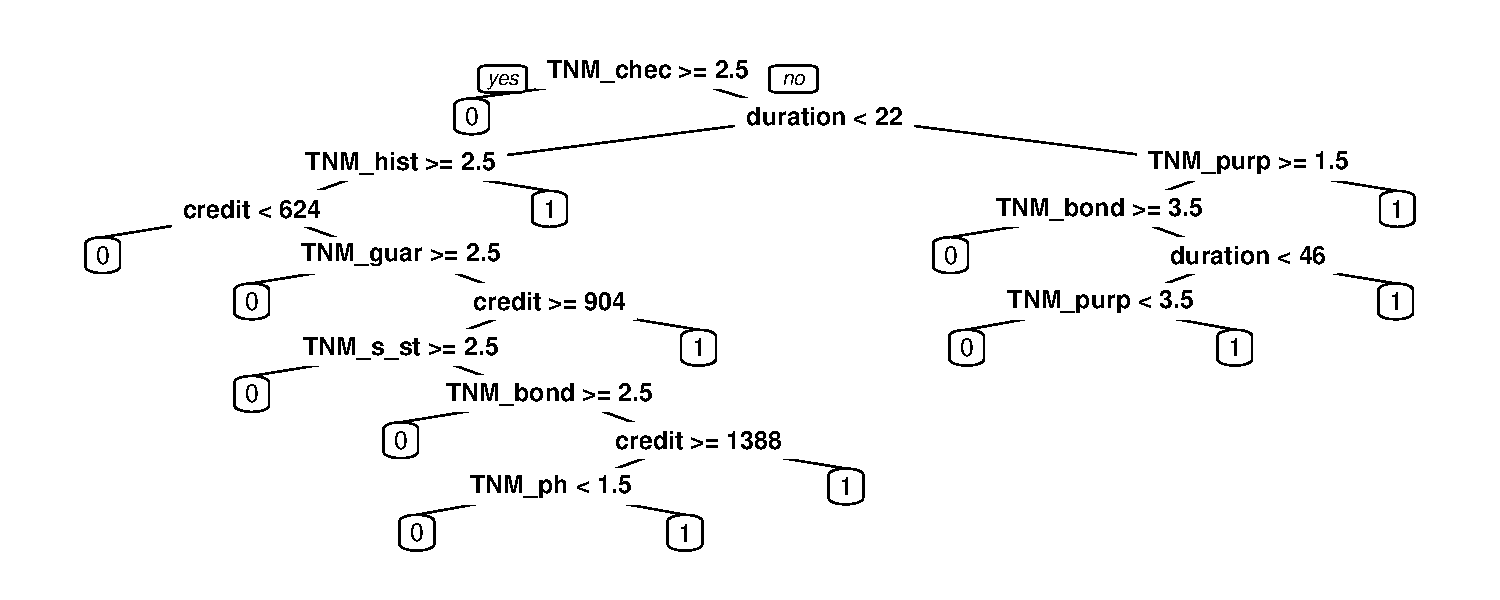
\includegraphics[width=\maxwidth]{figure/unnamed-chunk-36-1} \caption[Decision Tree Plot]{Decision Tree Plot}\label{fig:unnamed-chunk-36}
\end{figure}


\end{knitrout}
\textbf{Model Performance :} For evaluating the model performance, we generated confusion matrix for the Decision tree model. First generated the response from the model:
\begin{knitrout}
\definecolor{shadecolor}{rgb}{0.969, 0.969, 0.969}\color{fgcolor}\begin{kframe}
\begin{alltt}
\hlstd{pr} \hlkwb{<-} \hlkwd{predict}\hlstd{(rpart,} \hlkwc{newdata}\hlstd{=dataset[test,} \hlkwd{c}\hlstd{(input, target)],} \hlkwc{type}\hlstd{=}\hlstr{"class"}\hlstd{)}
\end{alltt}
\end{kframe}
\end{knitrout}
And the confusion matrix showing count is :
\begin{knitrout}
\definecolor{shadecolor}{rgb}{0.969, 0.969, 0.969}\color{fgcolor}\begin{kframe}
\begin{alltt}
\hlkwd{table}\hlstd{(dataset[test,} \hlkwd{c}\hlstd{(input, target)]}\hlopt{$}\hlstd{R01_credibility, pr,}
      \hlkwc{dnn}\hlstd{=}\hlkwd{c}\hlstd{(}\hlstr{"Actual"}\hlstd{,} \hlstr{"Predicted"}\hlstd{))}
\end{alltt}
\begin{verbatim}
##       Predicted
## Actual   0   1
##      0 124  21
##      1  23  32
\end{verbatim}
\end{kframe}
\end{knitrout}
Confusion matrix showing the proportions:


\begin{knitrout}
\definecolor{shadecolor}{rgb}{0.969, 0.969, 0.969}\color{fgcolor}\begin{kframe}
\begin{alltt}
\hlkwd{pcme}\hlstd{(dataset[test,} \hlkwd{c}\hlstd{(input, target)]}\hlopt{$}\hlstd{R01_credibility, pr)}
\end{alltt}
\begin{verbatim}
##       Predicted
## Actual    0    1 Error
##      0 0.62 0.10  0.14
##      1 0.12 0.16  0.42
\end{verbatim}
\end{kframe}
\end{knitrout}
From above error matrix we will get sensitivity and specificity proportion as (1-error) from first row and second row respectively. The overall error percentage is:


\begin{knitrout}
\definecolor{shadecolor}{rgb}{0.969, 0.969, 0.969}\color{fgcolor}\begin{kframe}
\begin{alltt}
\hlkwd{overall}\hlstd{(}\hlkwd{table}\hlstd{(pr, dataset[test,} \hlkwd{c}\hlstd{(input, target)]}\hlopt{$}\hlstd{R01_credibility,}
              \hlkwc{dnn}\hlstd{=}\hlkwd{c}\hlstd{(}\hlstr{"Predicted"}\hlstd{,} \hlstr{"Actual"}\hlstd{)))}
\end{alltt}
\begin{verbatim}
## 0.22
\end{verbatim}
\end{kframe}
\end{knitrout}
%<<echo=FALSE>>=
%avgerr <- function(x) 
%  cat(mean(c(x[1,2], x[2,1]) / apply(x, 1, sum))) 
%avgerr(table(pr, dataset[test, c(input, target)]$R01_credibility,  
%             dnn=c("Predicted", "Actual")))
%@
ROC curve for Decision tree model is shown in Figure [5]. The line right on the diagonal serves like a boundary between the good and bad models. The curve approaching to the top left hints a good fitting model.


\begin{knitrout}
\definecolor{shadecolor}{rgb}{0.969, 0.969, 0.969}\color{fgcolor}\begin{kframe}
\begin{alltt}
\hlkwd{print}\hlstd{(p)}
\end{alltt}
\end{kframe}\begin{figure}
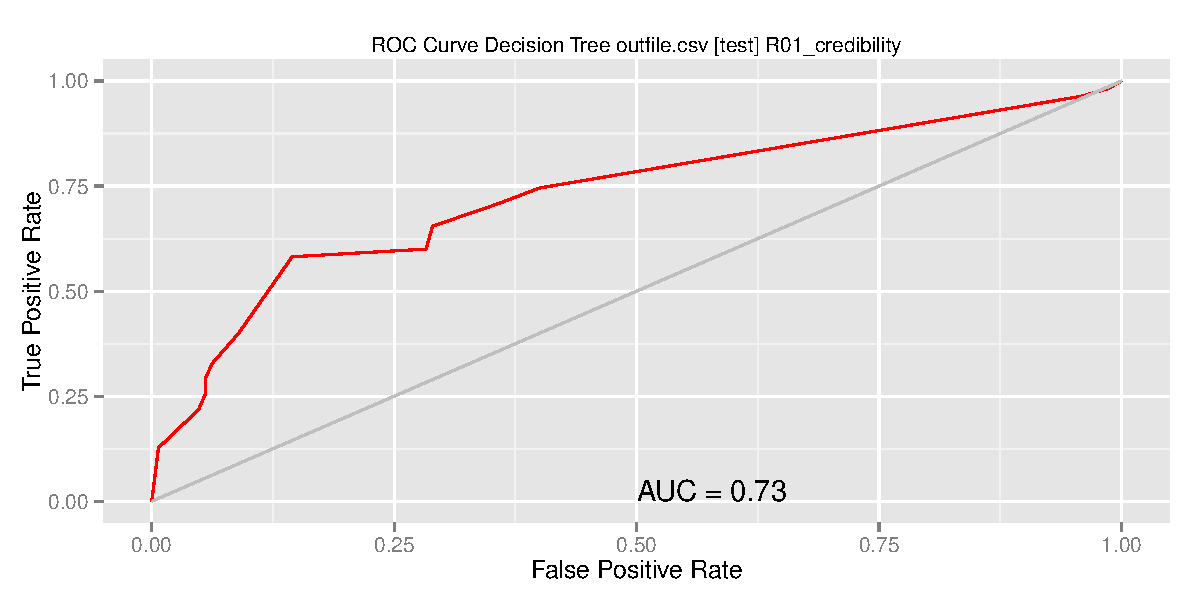
\includegraphics[width=\maxwidth]{figure/unnamed-chunk-44-1} \caption[ROC Curve-Decision Tree]{ROC Curve-Decision Tree}\label{fig:unnamed-chunk-44}
\end{figure}


\end{knitrout}
And the specificity/sensitivity plot is shown in Figure [6].


\begin{knitrout}
\definecolor{shadecolor}{rgb}{0.969, 0.969, 0.969}\color{fgcolor}\begin{kframe}
\begin{alltt}
\hlkwd{plot}\hlstd{(}\hlkwd{performance}\hlstd{(pred,} \hlstr{"sens"}\hlstd{,} \hlstr{"spec"}\hlstd{),} \hlkwc{col}\hlstd{=}\hlstr{"#CC0000FF"}\hlstd{,} \hlkwc{lty}\hlstd{=}\hlnum{1}\hlstd{,} \hlkwc{add}\hlstd{=}\hlnum{FALSE}\hlstd{)}
\end{alltt}
\end{kframe}\begin{figure}
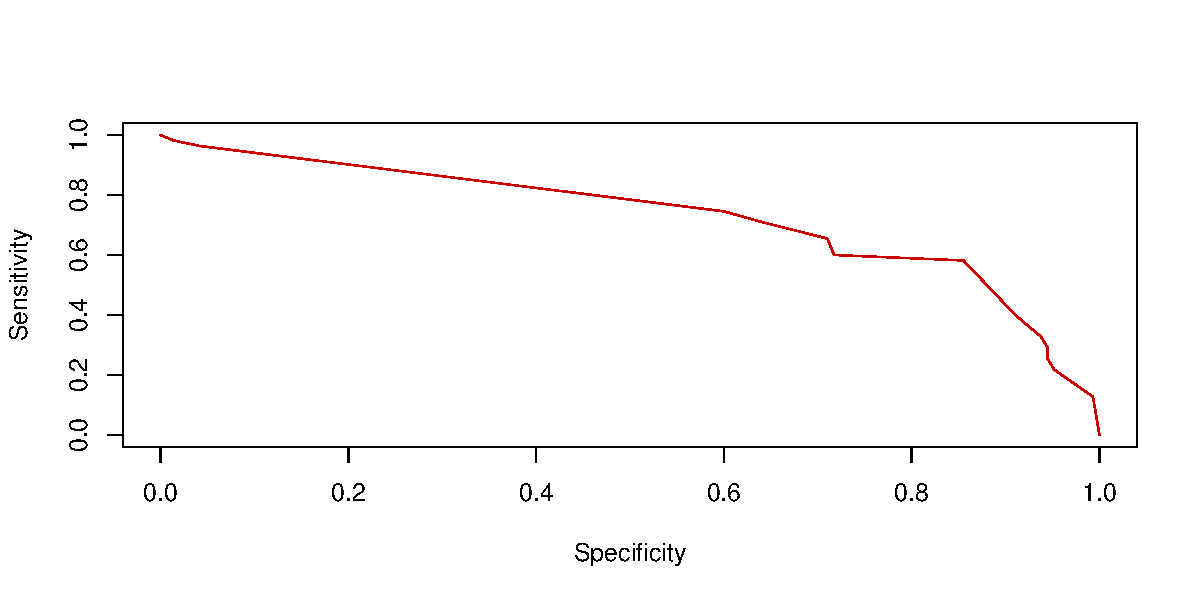
\includegraphics[width=\maxwidth]{figure/unnamed-chunk-46-1} \caption[Decision Tree - Sensitivity/Specificity Plot]{Decision Tree - Sensitivity/Specificity Plot}\label{fig:unnamed-chunk-46}
\end{figure}


\end{knitrout}
Thus the overall performance of Decision tree is analysed from above discussed measures. It is giving an accuracy of 78\%.\par
%%%%%%%%%%%%%%%%%%%%%%%%%%%%%%%%%%%%%%%%%%%%
Cross validation is a resampling approach which enables to obtain a more honest error rate estimate or average accuracy of the tree computed on the whole dataset. The cross validation consists to randomly split the data in K folds. We reiterate the following process, by turning the sub-samples: learning the model on (K-1) folds, computing performance measures on the fold number K. We observe that we have the same number of examples in each fold. We applied 10-fold cross validation on 1000 samples of the german credit dataset.
\begin{knitrout}
\definecolor{shadecolor}{rgb}{0.969, 0.969, 0.969}\color{fgcolor}\begin{kframe}
\begin{alltt}
\hlkwd{library}\hlstd{(rpart)}
\hlstd{dataset} \hlkwb{<-} \hlkwd{read.csv}\hlstd{(}\hlstr{"/home/freestyler/BDA_project/Data/outfile.csv"}\hlstd{)}
\hlstd{n}\hlkwb{<-}\hlkwd{nrow}\hlstd{(dataset)}
\hlstd{K}\hlkwb{<-}\hlnum{10}
\hlstd{divide}\hlkwb{<-} \hlstd{n} \hlopt \hlstd{K}
\hlkwd{set.seed}\hlstd{(}\hlnum{5}\hlstd{)}
\hlcom{#The runif() function can be used to simulate n independent uniform random variables.}
\hlstd{unirand}\hlkwb{<-}\hlkwd{runif}\hlstd{(n)}
\hlcom{#rank returns the lowest order of position, returns the sample ranks of the values in a vector.}
\hlstd{rang}\hlkwb{<-}\hlkwd{rank}\hlstd{(unirand)}
\hlstd{bloc}\hlkwb{<-}\hlstd{(rang} \hlopt{-} \hlnum{1}\hlstd{)}\hlopt\hlstd{divide} \hlopt{+}\hlnum{1}
\hlstd{bloc}\hlkwb{<-}\hlkwd{as.factor}\hlstd{(bloc)}
\hlkwd{print}\hlstd{(}\hlkwd{summary}\hlstd{(bloc))}
\end{alltt}
\begin{verbatim}
##   1   2   3   4   5   6   7   8   9  10 
## 100 100 100 100 100 100 100 100 100 100
\end{verbatim}
\end{kframe}
\end{knitrout}
We can repeat now the learning process and the test process. We collect each error rate,sensitivity, specificity in a vector.Printing Each sub-sample's of sensitivity ,specificity and accuracy:
\begin{knitrout}
\definecolor{shadecolor}{rgb}{0.969, 0.969, 0.969}\color{fgcolor}\begin{kframe}
\begin{verbatim}
##                  [,1]
## sensitivity 0.9305556
## sensitivity 0.8656716
## sensitivity 0.9027778
## sensitivity 0.9189189
## sensitivity 0.9014085
## sensitivity 0.9104478
## sensitivity 0.9090909
## sensitivity 0.8181818
## sensitivity 0.8589744
## sensitivity 0.8208955
##                  [,1]
## specificity 0.2500000
## specificity 0.3939394
## specificity 0.4642857
## specificity 0.3076923
## specificity 0.4482759
## specificity 0.4242424
## specificity 0.2941176
## specificity 0.4705882
## specificity 0.2272727
## specificity 0.4545455
##      [,1]
## acc1 0.74
## acc1 0.71
## acc1 0.78
## acc1 0.76
## acc1 0.77
## acc1 0.75
## acc1 0.70
## acc1 0.70
## acc1 0.72
## acc1 0.70
\end{verbatim}
\end{kframe}
\end{knitrout}
Because we have the same number of examples in each fold, we can compute unweighted mean. This is the average of each sub-sample's sensitivity:
\begin{knitrout}
\definecolor{shadecolor}{rgb}{0.969, 0.969, 0.969}\color{fgcolor}\begin{kframe}
\begin{verbatim}
## [1] 0.8836923
\end{verbatim}
\end{kframe}
\end{knitrout}
This is the average of each sub-sample's specificity:
\begin{knitrout}
\definecolor{shadecolor}{rgb}{0.969, 0.969, 0.969}\color{fgcolor}\begin{kframe}
\begin{verbatim}
## [1] 0.373496
\end{verbatim}
\end{kframe}
\end{knitrout}
This is the cross validation accuracy estimation:
\begin{knitrout}
\definecolor{shadecolor}{rgb}{0.969, 0.969, 0.969}\color{fgcolor}\begin{kframe}
\begin{verbatim}
## [1] 0.733
\end{verbatim}
\end{kframe}
\end{knitrout}
%%%%%%%%%%%%%%%%%%%%%%%%%%%%%%%%%%%%%%%%%%%%%%%%%%%%%%%%%



\subsection{Support Vector Machine}\hspace{0.9cm} Support Vector Machines are an excellent tool for classification. The goal of a support vector machine is to find  the optimal separating hyperplane which maximizes the margin of the training data. SVM is a classification algorithm, this will use to predict if something belongs to a particular class or not. Support Vector Machines was worked out for linear two-class classification with margin, where margin means the minimal distance from the separating hyperplane to the closest data points. SVM learning machine seeks for an optimal separating hyperplane, where the margin is maximal. An important and unique feature of this approach is that the solution is based only on those data points, which are at the margin. These points are called support vectors. For instance in Figure [7] we can see that there exists multiple lines that offer a solution to the problem. A line is bad if it passes too close to the points because it will be noise sensitive and it will not generalize correctly. The operation of the SVM algorithm is based on finding the hyperplane that gives the largest minimum distance to the training examples.

\begin{figure}[h]
\begin{center}
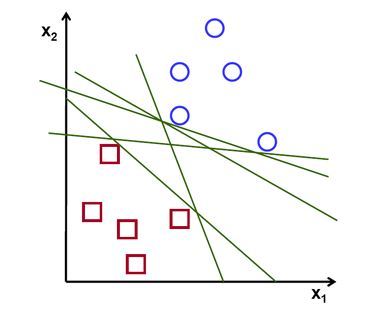
\includegraphics [scale=0.75]{svm.JPG}
\end{center}
\caption{Linearly separable set of 2D-points which belong to one of two classes}
\end{figure}

Notation of hyperplane is:

\hspace{5cm}\begin{equation} \label{eq:hyper_plane}
f(x)= \beta_0 + \beta^T X.
\end{equation}

where $\beta$ is known as the weight vector and $\beta_{0}$ as the bias.

The optimal hyperplane can be represented in an infinite number of different
ways by scaling of $\beta$ and $\beta_{0}$. As a matter of convention, among all the
possible representations of the hyperplane, the one chosen is:


\hspace{5cm}\begin{equation} \label{eq:hyperplane}
|\beta_0 + \beta^T X|=1.
\end{equation}

\par Where x symbolizes the training examples closest to the hyperplane.Geometry that gives the distance between a point x and a hyperplane ($\beta$, $\beta_{0}$):

\hspace{5cm}
\begin{equation} \label{eq:dist}
distance = \frac{\beta_0 + \beta^T X|}{||\beta||}
\end{equation}

\par Training set that is closest to the hyperplane is called support vectors. This representation is known as the canonical hyperplane.For the canonical hyperplane, the numerator is equal to one and the distance to the support vectors is:
\hspace{5cm}
\begin{equation} \label{eq:distsv}
distance_{support vectors}=\frac{\beta_0 + \beta^T X|}{||\beta||} = \frac{1}{||\beta||}.
\end{equation}

\par Margin M, is twice the distance to the closest examples:
\hspace{5cm} 
\begin{equation} \label{eq:margin}
M= \frac{2}{||\beta||}
\end{equation}

The problem of maximizing M is equivalent to the problem of minimizing a 
function L($\beta$) subject to some constraints. The constraints model the 
requirement for the hyperplane to classify correctly all the training examples x_{i}.

\hspace{5cm}
\begin{equation} \label{eq:sample}
min_{\beta,\beta_0}L(\beta) = \frac{1}{2} || \beta^2 ||  (\beta^Tx_i + \beta_0)>=1\forall_i.
\end{equation}

So as mentioned earlier the objective is to find the classifier with the best margin of separation. SVM can be implemented with R using the command ksvm() in the R package \textit{kernlab}.

\begin{knitrout}
\definecolor{shadecolor}{rgb}{0.969, 0.969, 0.969}\color{fgcolor}\begin{kframe}
\begin{alltt}
\hlkwd{library}\hlstd{(kernlab,} \hlkwc{quietly}\hlstd{=}\hlnum{TRUE}\hlstd{)}
\hlstd{ksvm} \hlkwb{<-} \hlkwd{ksvm}\hlstd{(}\hlkwd{as.factor}\hlstd{(R01_credibility)} \hlopt{~} \hlstd{.,}
                 \hlkwc{data}\hlstd{=dataset[train,}\hlkwd{c}\hlstd{(input, target)],}
                 \hlkwc{kernel}\hlstd{=}\hlstr{"rbfdot"}\hlstd{,}
                 \hlkwc{prob.model}\hlstd{=}\hlnum{TRUE}\hlstd{)}
\end{alltt}
\end{kframe}
\end{knitrout}
\begin{knitrout}
\definecolor{shadecolor}{rgb}{0.969, 0.969, 0.969}\color{fgcolor}\begin{kframe}
\begin{alltt}
\hlstd{ksvm}
\end{alltt}
\begin{verbatim}
## Support Vector Machine object of class "ksvm" 
## 
## SV type: C-svc  (classification) 
##  parameter : cost C = 1 
## 
## Gaussian Radial Basis kernel function. 
##  Hyperparameter : sigma =  0.0361190834923943 
## 
## Number of Support Vectors : 492 
## 
## Objective Function Value : -380.6035 
## Training error : 0.175 
## Probability model included.
\end{verbatim}
\end{kframe}
\end{knitrout}
Then using predict function and test data generate the predicted values. ROC Curve for this model is shown in Figure [8].
\begin{knitrout}
\definecolor{shadecolor}{rgb}{0.969, 0.969, 0.969}\color{fgcolor}\begin{kframe}
\begin{alltt}
\hlkwd{library}\hlstd{(ROCR)}
\hlkwd{library}\hlstd{(ggplot2,} \hlkwc{quietly}\hlstd{=}\hlnum{TRUE}\hlstd{)}
\hlstd{pr} \hlkwb{<-} \hlkwd{predict}\hlstd{(ksvm,} \hlkwc{newdata}\hlstd{=}\hlkwd{na.omit}\hlstd{(dataset[test,} \hlkwd{c}\hlstd{(input, target)]),}
            \hlkwc{type}\hlstd{=}\hlstr{"probabilities"}\hlstd{)[,}\hlnum{2}\hlstd{]}
\end{alltt}
\end{kframe}
\end{knitrout}

\begin{knitrout}
\definecolor{shadecolor}{rgb}{0.969, 0.969, 0.969}\color{fgcolor}\begin{kframe}
\begin{alltt}
\hlkwd{print}\hlstd{(p)}
\end{alltt}
\end{kframe}\begin{figure}
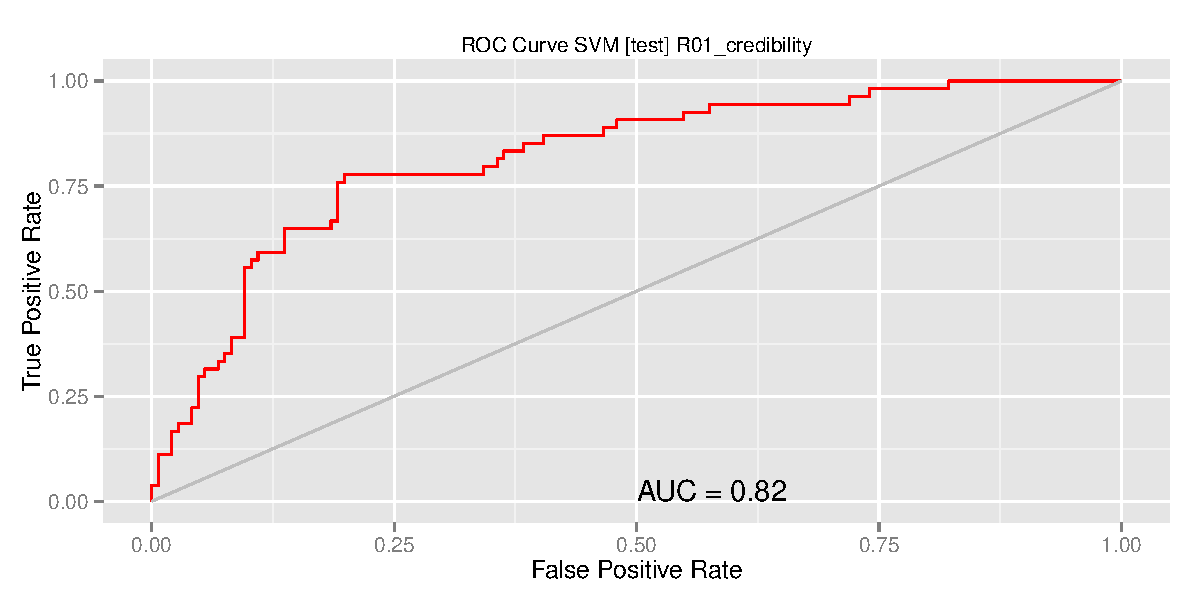
\includegraphics[width=\maxwidth]{figure/unnamed-chunk-57-1} \caption[ROC Curve - Support Vector Machine]{ROC Curve - Support Vector Machine}\label{fig:unnamed-chunk-57}
\end{figure}


\end{knitrout}
The confusion matrix showing the counts and error proportion is given below:
\begin{knitrout}
\definecolor{shadecolor}{rgb}{0.969, 0.969, 0.969}\color{fgcolor}\begin{kframe}
\begin{alltt}
\hlstd{pr} \hlkwb{<-} \hlkwd{predict}\hlstd{(ksvm,} \hlkwc{newdata}\hlstd{=}\hlkwd{na.omit}\hlstd{(dataset[test,} \hlkwd{c}\hlstd{(input, target)]))}
\hlkwd{table}\hlstd{(dataset[test,} \hlkwd{c}\hlstd{(input, target)]}\hlopt{$}\hlstd{R01_credibility, pr,}
      \hlkwc{dnn}\hlstd{=}\hlkwd{c}\hlstd{(}\hlstr{"Actual"}\hlstd{,} \hlstr{"Predicted"}\hlstd{))}
\end{alltt}
\begin{verbatim}
##       Predicted
## Actual   0   1
##      0 132  14
##      1  27  27
\end{verbatim}
\end{kframe}
\end{knitrout}

\begin{knitrout}
\definecolor{shadecolor}{rgb}{0.969, 0.969, 0.969}\color{fgcolor}\begin{kframe}
\begin{verbatim}
##       Predicted
## Actual    0    1 Error
##      0 0.66 0.07   0.1
##      1 0.14 0.14   0.5
\end{verbatim}
\end{kframe}
\end{knitrout}
Thus the Support vector machine model giving an accuracy of 79.5\%, sensitivity proportion 0.9 but specificity proportion 0.5 only.\par
%%%%%%%%%%%%%%%%%%%%%%%%%%%%%%%%%%%%%%%%%%%%%%%%%%%%%%%%%%%%%%%%%%%%%%%%
We observe that we have the same number of examples in each fold like in previous models we are applying 10 fold cross validation. We can repeat now the learning process and the test process. We collect each measure in a vector.




\begin{knitrout}
\definecolor{shadecolor}{rgb}{0.969, 0.969, 0.969}\color{fgcolor}\begin{kframe}
\begin{alltt}
\hlkwa{for}\hlstd{(k} \hlkwa{in} \hlnum{1}\hlopt{:}\hlstd{K)\{}
\hlstd{ksvm1} \hlkwb{<-} \hlkwd{ksvm}\hlstd{(}\hlkwd{as.factor}\hlstd{(R01_credibility)} \hlopt{~}\hlstd{.,} \hlkwc{data} \hlstd{= dataset[bloc}\hlopt{!=}\hlstd{k,],}\hlkwc{probability}\hlstd{=}\hlnum{TRUE}\hlstd{)}
\hlstd{pred} \hlkwb{<-} \hlkwd{predict}\hlstd{(ksvm1,}\hlkwc{newdata} \hlstd{=} \hlkwd{na.omit}\hlstd{(dataset[bloc}\hlopt{==}\hlstd{k,]))}
\hlcom{#confusion matrix for each partition}
\hlstd{mc}\hlkwb{<-}\hlkwd{table}\hlstd{(dataset}\hlopt{$}\hlstd{R01_credibility[bloc}\hlopt{==}\hlstd{k],pred)}
\hlstd{err}\hlkwb{<-}\hlnum{1.0} \hlopt{-} \hlstd{(mc[}\hlnum{1}\hlstd{,}\hlnum{1}\hlstd{]}\hlopt{+}\hlstd{mc[}\hlnum{2}\hlstd{,}\hlnum{2}\hlstd{])}\hlopt{/}\hlkwd{sum}\hlstd{(mc)}
\hlstd{acc1}\hlkwb{<-}\hlnum{1}\hlopt{-}\hlstd{(err)}
\hlstd{a}\hlkwb{<-}\hlstd{mc[}\hlnum{1}\hlstd{,}\hlnum{1}\hlstd{]}
\hlstd{b}\hlkwb{<-}\hlstd{mc[}\hlnum{1}\hlstd{,}\hlnum{1}\hlstd{]}\hlopt{+}\hlstd{mc[}\hlnum{1}\hlstd{,}\hlnum{2}\hlstd{]}
\hlstd{sensitivity}\hlkwb{<-}\hlstd{a}\hlopt{/}\hlstd{b}
\hlstd{c}\hlkwb{<-}\hlstd{mc[}\hlnum{2}\hlstd{,}\hlnum{2}\hlstd{]}
\hlstd{d}\hlkwb{<-}\hlstd{mc[}\hlnum{2}\hlstd{,}\hlnum{2}\hlstd{]}\hlopt{+}\hlstd{mc[}\hlnum{2}\hlstd{,}\hlnum{1}\hlstd{]}
\hlstd{specificity}\hlkwb{<-}\hlstd{c}\hlopt{/}\hlstd{d}
\hlstd{all.sense}\hlkwb{<-}\hlkwd{rbind}\hlstd{(all.sense,sensitivity)}
\hlstd{all.spese}\hlkwb{<-}\hlkwd{rbind}\hlstd{(all.spese,specificity)}
\hlstd{all.acc1}\hlkwb{<-}\hlkwd{rbind}\hlstd{(all.acc1,acc1)}
\hlstd{\}}
\end{alltt}
\end{kframe}
\end{knitrout}

\begin{knitrout}
\definecolor{shadecolor}{rgb}{0.969, 0.969, 0.969}\color{fgcolor}\begin{kframe}
\begin{verbatim}
##                  [,1]
## sensitivity 0.8888889
## sensitivity 0.9402985
## sensitivity 0.9166667
## sensitivity 0.9324324
## sensitivity 0.9154930
## sensitivity 0.9402985
## sensitivity 0.9242424
## sensitivity 0.8787879
## sensitivity 0.8717949
## sensitivity 0.8805970
##                  [,1]
## specificity 0.3928571
## specificity 0.4545455
## specificity 0.4642857
## specificity 0.3846154
## specificity 0.5862069
## specificity 0.3939394
## specificity 0.3529412
## specificity 0.4705882
## specificity 0.2727273
## specificity 0.3939394
##      [,1]
## acc1 0.75
## acc1 0.78
## acc1 0.79
## acc1 0.79
## acc1 0.82
## acc1 0.76
## acc1 0.73
## acc1 0.74
## acc1 0.74
## acc1 0.72
\end{verbatim}
\end{kframe}
\end{knitrout}
Because we have the same number of examples in each fold, we can compute unweighted mean. This is the average of each sub-sample's sensitivity:
\begin{knitrout}
\definecolor{shadecolor}{rgb}{0.969, 0.969, 0.969}\color{fgcolor}\begin{kframe}
\begin{verbatim}
## [1] 0.90895
\end{verbatim}
\end{kframe}
\end{knitrout}
This is the average of each sub-sample's specificity:
\begin{knitrout}
\definecolor{shadecolor}{rgb}{0.969, 0.969, 0.969}\color{fgcolor}\begin{kframe}
\begin{verbatim}
## [1] 0.4166646
\end{verbatim}
\end{kframe}
\end{knitrout}
This is the cross validation accuracy estimation:
\begin{knitrout}
\definecolor{shadecolor}{rgb}{0.969, 0.969, 0.969}\color{fgcolor}\begin{kframe}
\begin{verbatim}
## [1] 0.762
\end{verbatim}
\end{kframe}
\end{knitrout}
%%%%%%%%%%%%%%%%%%%%%%%%%%%%%%%%%%%%%%%%%%%%5

\subsection{Neural Network}\hspace{0.9cm}Neural networks comprise yet another group of nonlinear procedures for prediction and classification. Neural networks are computational analogs of the processes that describe the working of neurons. Neural nets consist of connected input and output layers, each containing numerous units, where the connections among the units of the layers have weights associated with them. A multilayer neural network consists of an input layer of distinct units (usually input units represent the attributes of the case that needs to be classified), one or more hidden layers, and an output layer with several units that represent the class that needs to be predicted. Each layer is made up of several units. The inputs from the units of the first layer are weighted and fed simultaneously to a second layer of neuron-like units, known as the hidden layer. Each of its units takes as its input a weighted sum of the outputs
of the previous layer and applies a nonlinear activation function to determine its output. The activation function is usually a logistic function that transforms the output to a number that is between 0 and 1; for this reason, it is often referred to as the squashing function. The output units may already be the actual output of the system (in which case we talk about a single hidden layer), or the outputs of the
first hidden layer can be fed as inputs to another hidden layer (in which case we have two hidden layers), and so on if additional hidden layers are involved.\par
\hspace{0.5cm} One needs to decide on the number of hidden layers and the number of units in the various layers, as well as the weights that connect the inputs and outputs of these layers. Neural nets are very general, and because of the nonlinear activation functions neural nets are able to approximate most nonlinear functional relationships very well. Of course, the weights in these systems have to be estimated by training the system on actual data. The iterative method of back-propagation can be used to determine the empirical weights that lead to the best fit on a given training sample. For that, one needs to specify a learning parameter that controls the speed of convergence of this iterative estimation method.\par
\hspace{0.5cm} One disadvantage of neural nets is that the approximating models relating inputs and outputs are purely "black box'' models, and they provide very little insight into what these models really do. Also, the user of neural nets must make many modeling assumptions, such as the number of hidden layers and the number of units in each hidden layer, and usually there is little guidance on how to do this. It takes considerable experience to find the most appropriate representation. The package \textit{nnet} is used here\cite{[7]}.\par

The Neural network model using nnet package is build:
\begin{knitrout}
\definecolor{shadecolor}{rgb}{0.969, 0.969, 0.969}\color{fgcolor}\begin{kframe}
\begin{alltt}
\hlkwd{library}\hlstd{(nnet,} \hlkwc{quietly}\hlstd{=}\hlnum{TRUE}\hlstd{)}

\hlkwd{set.seed}\hlstd{(}\hlnum{199}\hlstd{)}
\hlstd{nnet} \hlkwb{<-} \hlkwd{nnet}\hlstd{(}\hlkwd{as.factor}\hlstd{(R01_credibility)} \hlopt{~} \hlstd{.,}
                 \hlkwc{data}\hlstd{=dataset[sample,}\hlkwd{c}\hlstd{(input, target)],}
                 \hlkwc{size}\hlstd{=}\hlnum{7}\hlstd{,} \hlkwc{skip}\hlstd{=}\hlnum{TRUE}\hlstd{,} \hlkwc{MaxNWts}\hlstd{=}\hlnum{10000}\hlstd{,} \hlkwc{trace}\hlstd{=}\hlnum{FALSE}\hlstd{,} \hlkwc{maxit}\hlstd{=}\hlnum{100}\hlstd{)}
\end{alltt}
\end{kframe}
\end{knitrout}
The result of the modelling is :
\begin{knitrout}
\definecolor{shadecolor}{rgb}{0.969, 0.969, 0.969}\color{fgcolor}\begin{kframe}
\begin{verbatim}
## A 18-7-1 network with 159 weights.
## Output: as.factor(R01_credibility).
## Sum of Squares Residuals: 41.3214.
\end{verbatim}
\end{kframe}
\end{knitrout}
\begin{knitrout}
\definecolor{shadecolor}{rgb}{0.969, 0.969, 0.969}\color{fgcolor}\begin{kframe}
\begin{alltt}
\hlkwd{print}\hlstd{(}\hlkwd{summary}\hlstd{(nnet))}
\end{alltt}
\begin{verbatim}
## Neural Network build options: skip-layer connections; entropy fitting.
## 
## In the following table:
##    b  represents the bias associated with a node
##    h1 represents hidden layer node 1
##    i1 represents input node 1 (i.e., input variable 1)
##    o  represents the output node
## 
## Weights for node h1:
##   b->h1  i1->h1  i2->h1  i3->h1  i4->h1  i5->h1  i6->h1  i7->h1  i8->h1 
##  -17.61    8.21   39.25   -3.06  -22.45    3.17    2.21   -1.37    1.08 
##  i9->h1 i10->h1 i11->h1 i12->h1 i13->h1 i14->h1 i15->h1 i16->h1 i17->h1 
##    0.21   11.62    5.64  -18.04    2.67  -17.93   -0.42    5.55   -3.50 
## i18->h1 
##  -10.84 
## 
## Weights for node h2:
##   b->h2  i1->h2  i2->h2  i3->h2  i4->h2  i5->h2  i6->h2  i7->h2  i8->h2 
##    3.69   -3.82    7.44   -4.46    3.67    4.50    5.36    1.85   16.08 
##  i9->h2 i10->h2 i11->h2 i12->h2 i13->h2 i14->h2 i15->h2 i16->h2 i17->h2 
##    7.22    8.77   -9.37   -3.38   20.61   -0.76   20.55    0.54   17.97 
## i18->h2 
##   -4.14 
## 
## Weights for node h3:
##   b->h3  i1->h3  i2->h3  i3->h3  i4->h3  i5->h3  i6->h3  i7->h3  i8->h3 
##    4.03   29.54    5.60    1.67  -14.70   10.29    9.72   14.08   -4.25 
##  i9->h3 i10->h3 i11->h3 i12->h3 i13->h3 i14->h3 i15->h3 i16->h3 i17->h3 
##   -4.83    0.89    0.09  -23.48   10.57   -7.15   -8.43   11.59    0.71 
## i18->h3 
##    2.54 
## 
## Weights for node h4:
##   b->h4  i1->h4  i2->h4  i3->h4  i4->h4  i5->h4  i6->h4  i7->h4  i8->h4 
##   11.70    4.36   12.76   11.72    6.57   15.23    3.50   -7.24   39.54 
##  i9->h4 i10->h4 i11->h4 i12->h4 i13->h4 i14->h4 i15->h4 i16->h4 i17->h4 
##  -11.78   -7.63   -9.42   -3.56   -0.60  -14.00    5.71    8.61   12.65 
## i18->h4 
##   -8.92 
## 
## Weights for node h5:
##   b->h5  i1->h5  i2->h5  i3->h5  i4->h5  i5->h5  i6->h5  i7->h5  i8->h5 
##    3.17   -0.82   23.11    8.37    2.56    5.12  -14.45   -0.15   31.72 
##  i9->h5 i10->h5 i11->h5 i12->h5 i13->h5 i14->h5 i15->h5 i16->h5 i17->h5 
##   -7.03  -10.73    1.39   -9.58    4.12  -42.00    7.66   11.44    6.00 
## i18->h5 
##   -7.19 
## 
## Weights for node h6:
##   b->h6  i1->h6  i2->h6  i3->h6  i4->h6  i5->h6  i6->h6  i7->h6  i8->h6 
##   -8.26   -8.20    6.96   23.23   -2.50    6.83    7.10  -20.09   -7.52 
##  i9->h6 i10->h6 i11->h6 i12->h6 i13->h6 i14->h6 i15->h6 i16->h6 i17->h6 
##   20.61   -7.99    2.24   -7.59   20.47  -16.77    4.87  -16.66   13.21 
## i18->h6 
##  -11.23 
## 
## Weights for node h7:
##   b->h7  i1->h7  i2->h7  i3->h7  i4->h7  i5->h7  i6->h7  i7->h7  i8->h7 
##   13.33  -37.31   30.45   -8.37   -7.88    9.32    3.32  -28.75    8.92 
##  i9->h7 i10->h7 i11->h7 i12->h7 i13->h7 i14->h7 i15->h7 i16->h7 i17->h7 
##   12.83   10.51  -15.35  -13.05    3.55   -1.41    7.22    4.05    9.33 
## i18->h7 
##   14.62 
## 
## Weights for node o:
##   b->o  h1->o  h2->o  h3->o  h4->o  h5->o  h6->o  h7->o  i1->o  i2->o 
##   8.19  -7.13  -7.55  -7.37 -11.69  14.46   6.41  -8.55   1.85   2.14 
##  i3->o  i4->o  i5->o  i6->o  i7->o  i8->o  i9->o i10->o i11->o i12->o 
##  -1.33  -2.03   2.18  -0.26  -1.47   1.31  -1.39   1.64  -2.97  -2.59 
## i13->o i14->o i15->o i16->o i17->o i18->o 
##   1.85   0.16   0.34   1.75   0.56  -0.08
\end{verbatim}
\end{kframe}
\end{knitrout}
Now evaluating the model performance. At first take the response from the model then generate the Confusion matrix for the Neural Network model.
\begin{knitrout}
\definecolor{shadecolor}{rgb}{0.969, 0.969, 0.969}\color{fgcolor}\begin{kframe}
\begin{alltt}
\hlstd{pr} \hlkwb{<-} \hlkwd{predict}\hlstd{(nnet,} \hlkwc{newdata}\hlstd{=dataset[test,} \hlkwd{c}\hlstd{(input, target)],} \hlkwc{type}\hlstd{=}\hlstr{"class"}\hlstd{)}
\hlkwd{table}\hlstd{(dataset[test,} \hlkwd{c}\hlstd{(input, target)]}\hlopt{$}\hlstd{R01_credibility, pr,}
      \hlkwc{dnn}\hlstd{=}\hlkwd{c}\hlstd{(}\hlstr{"Actual"}\hlstd{,} \hlstr{"Predicted"}\hlstd{))}
\end{alltt}
\begin{verbatim}
##       Predicted
## Actual   0   1
##      0 110  35
##      1  27  28
\end{verbatim}
\end{kframe}
\end{knitrout}

\begin{knitrout}
\definecolor{shadecolor}{rgb}{0.969, 0.969, 0.969}\color{fgcolor}\begin{kframe}
\begin{alltt}
\hlstd{per} \hlkwb{<-} \hlkwd{pcme}\hlstd{(dataset[test,} \hlkwd{c}\hlstd{(input, target)]}\hlopt{$}\hlstd{R01_credibility, pr)}
\hlkwd{round}\hlstd{(per,} \hlnum{2}\hlstd{)}
\end{alltt}
\begin{verbatim}
##       Predicted
## Actual    0    1 Error
##      0 0.55 0.18  0.24
##      1 0.14 0.14  0.49
\end{verbatim}
\end{kframe}
\end{knitrout}
The ROC curve generated for the model is in Figure [9].


\begin{knitrout}
\definecolor{shadecolor}{rgb}{0.969, 0.969, 0.969}\color{fgcolor}\begin{kframe}
\begin{alltt}
\hlkwd{print}\hlstd{(p)}
\end{alltt}
\end{kframe}\begin{figure}
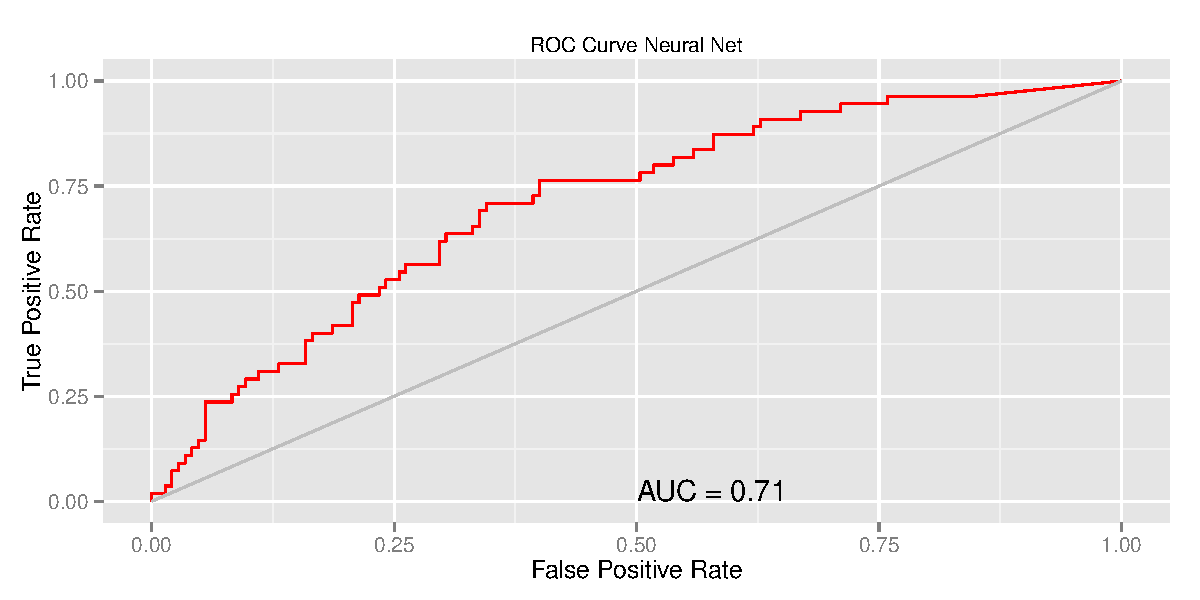
\includegraphics[width=\maxwidth]{figure/unnamed-chunk-75-1} \caption[ROC Curve - Neural Networks]{ROC Curve - Neural Networks}\label{fig:unnamed-chunk-75}
\end{figure}


\end{knitrout}
The model was giving an accuracy percentage of 69 only.\par
%%%%%%%%%%%%%%%%%%%%%%%%%%%%%%%%%%%%%%%%
The 10 fold cross validation with this model results:
\begin{knitrout}
\definecolor{shadecolor}{rgb}{0.969, 0.969, 0.969}\color{fgcolor}\begin{kframe}
\begin{verbatim}
##   1   2   3   4   5   6   7   8   9  10 
## 100 100 100 100 100 100 100 100 100 100
\end{verbatim}
\end{kframe}
\end{knitrout}
Repeating the learning process and the test process. Then collect each sensitivity,specificity, and accuracy in a vector. Printing each sub-sample's sensitivity, specificity and accuracy:
\begin{knitrout}
\definecolor{shadecolor}{rgb}{0.969, 0.969, 0.969}\color{fgcolor}\begin{kframe}
\begin{verbatim}
##                  [,1]
## sensitivity 0.8194444
## sensitivity 0.8059701
## sensitivity 0.8055556
## sensitivity 0.7702703
## sensitivity 0.7887324
## sensitivity 0.8507463
## sensitivity 0.7727273
## sensitivity 0.8030303
## sensitivity 0.7564103
## sensitivity 0.7761194
##                  [,1]
## specificity 0.4642857
## specificity 0.3939394
## specificity 0.3571429
## specificity 0.5000000
## specificity 0.5862069
## specificity 0.4545455
## specificity 0.5294118
## specificity 0.4117647
## specificity 0.4090909
## specificity 0.3636364
##      [,1]
## acc1 0.72
## acc1 0.67
## acc1 0.68
## acc1 0.70
## acc1 0.73
## acc1 0.72
## acc1 0.69
## acc1 0.67
## acc1 0.68
## acc1 0.64
\end{verbatim}
\end{kframe}
\end{knitrout}
Because we have the same number of examples in each fold, we can compute unweighted mean. This is the average of each sub-sample's sensitivity:
\begin{knitrout}
\definecolor{shadecolor}{rgb}{0.969, 0.969, 0.969}\color{fgcolor}\begin{kframe}
\begin{verbatim}
## [1] 0.7949006
\end{verbatim}
\end{kframe}
\end{knitrout}
This is the average of each sub-sample's specificity:
\begin{knitrout}
\definecolor{shadecolor}{rgb}{0.969, 0.969, 0.969}\color{fgcolor}\begin{kframe}
\begin{verbatim}
## [1] 0.4470024
\end{verbatim}
\end{kframe}
\end{knitrout}
This is the cross validation average accuracy:
\begin{knitrout}
\definecolor{shadecolor}{rgb}{0.969, 0.969, 0.969}\color{fgcolor}\begin{kframe}
\begin{verbatim}
## [1] 0.69
\end{verbatim}
\end{kframe}
\end{knitrout}
%%%%%%%%%%%%%%%%%%%%%%%%%%%%%%%%%%%%%%%%%%%%%%%%%%%%%%%%%%%%%%%%%%%%%

\subsubsection{PCA with Neural network} In this model we are doing PCA in the dataset and use it in the neural network model. For that purpose library \textit{caret} we are using.\par\\ 


\begin{knitrout}
\definecolor{shadecolor}{rgb}{0.969, 0.969, 0.969}\color{fgcolor}\begin{kframe}
\begin{alltt}
\hlstd{dataset} \hlkwb{<-} \hlkwd{read.csv}\hlstd{(}\hlstr{"/home/freestyler/outfile.csv"}\hlstd{,} \hlkwc{na.strings}\hlstd{=}\hlkwd{c}\hlstd{(}\hlstr{"."}\hlstd{,} \hlstr{"NA"}\hlstd{,} \hlstr{""}\hlstd{,} \hlstr{"?"}\hlstd{),} \hlkwc{strip.white}\hlstd{=}\hlnum{TRUE}\hlstd{,} \hlkwc{encoding}\hlstd{=}\hlstr{"UTF-8"}\hlstd{)}
\end{alltt}
\end{kframe}
\end{knitrout}

\begin{knitrout}
\definecolor{shadecolor}{rgb}{0.969, 0.969, 0.969}\color{fgcolor}\begin{kframe}
\begin{alltt}
\hlkwd{set.seed}\hlstd{(crv}\hlopt{$}\hlstd{seed)}
\hlstd{nobs} \hlkwb{<-} \hlkwd{nrow}\hlstd{(dataset)} \hlcom{# 1000 observations }
\hlstd{sample} \hlkwb{<-} \hlstd{train} \hlkwb{<-} \hlkwd{sample}\hlstd{(}\hlkwd{nrow}\hlstd{(dataset),} \hlnum{0.7}\hlopt{*}\hlstd{nobs)} \hlcom{# 700 observations}
\hlstd{validate} \hlkwb{<-} \hlkwd{sample}\hlstd{(}\hlkwd{setdiff}\hlstd{(}\hlkwd{seq_len}\hlstd{(}\hlkwd{nrow}\hlstd{(dataset)), train),} \hlnum{0.15}\hlopt{*}\hlstd{nobs)} \hlcom{# 150 observations}
\hlstd{test} \hlkwb{<-} \hlkwd{setdiff}\hlstd{(}\hlkwd{setdiff}\hlstd{(}\hlkwd{seq_len}\hlstd{(}\hlkwd{nrow}\hlstd{(dataset)), train), validate)} \hlcom{# 150 observations}
\end{alltt}
\end{kframe}
\end{knitrout}

\begin{knitrout}
\definecolor{shadecolor}{rgb}{0.969, 0.969, 0.969}\color{fgcolor}\begin{kframe}
\begin{alltt}
\hlkwd{set.seed}\hlstd{(}\hlnum{42}\hlstd{)}
\hlstd{nobs} \hlkwb{<-} \hlkwd{nrow}\hlstd{(dataset)} \hlcom{# 1000 observations}
\hlstd{train} \hlkwb{<-} \hlkwd{sample}\hlstd{(}\hlkwd{nrow}\hlstd{(dataset),} \hlnum{0.8}\hlopt{*}\hlstd{nobs)} \hlcom{# 800 observations}
\hlstd{validate} \hlkwb{<-} \hlkwa{NULL}
\hlstd{test} \hlkwb{<-} \hlkwd{setdiff}\hlstd{(}\hlkwd{setdiff}\hlstd{(}\hlkwd{seq_len}\hlstd{(}\hlkwd{nrow}\hlstd{(dataset)), train), validate)} \hlcom{# 200 observations}
\end{alltt}
\end{kframe}
\end{knitrout}



\begin{knitrout}
\definecolor{shadecolor}{rgb}{0.969, 0.969, 0.969}\color{fgcolor}\begin{kframe}
\begin{alltt}
\hlstd{xtrain} \hlkwb{<-} \hlstd{dataset[train,]}
\hlstd{xnew} \hlkwb{<-} \hlstd{dataset[}\hlopt{-}\hlstd{train,]}
\hlstd{ytrain} \hlkwb{<-} \hlstd{dataset}\hlopt{$}\hlstd{R01_credibility[train]}
\hlstd{ynew} \hlkwb{<-} \hlstd{dataset}\hlopt{$}\hlstd{R01_credibility[}\hlopt{-}\hlstd{train]}
\end{alltt}
\end{kframe}
\end{knitrout}
\hspace{0.5cm} The function first will run principal component analysis on the data. The cumulative percentage of variance is computed for each principal component. The function uses the thresh argument to determine how many components must be retained to capture this amount of variance in the predictors. Here we used threshold value as 0.95, the model description is given below.\\
\begin{knitrout}
\definecolor{shadecolor}{rgb}{0.969, 0.969, 0.969}\color{fgcolor}\begin{kframe}
\begin{alltt}
\hlkwd{library}\hlstd{(caret)}
\hlstd{modelFit} \hlkwb{<-} \hlkwd{pcaNNet}\hlstd{(xtrain[,} \hlnum{1}\hlopt{:}\hlnum{20}\hlstd{], ytrain,} \hlkwc{thresh}\hlstd{=}\hlnum{0.95}\hlstd{,}\hlkwc{size} \hlstd{=} \hlnum{5}\hlstd{,} \hlkwc{linout} \hlstd{=} \hlnum{TRUE}\hlstd{,} \hlkwc{trace} \hlstd{=} \hlnum{FALSE}\hlstd{)}
\hlstd{modelFit}
\end{alltt}
\begin{verbatim}
## Neural Network Model with PCA Pre-Processing
## 
## Created from 800 samples and 20 variables
## PCA needed 18 components to capture 95 percent of the variance
## 
## a 18-5-1 network with 101 weights
## options were - linear output units
\end{verbatim}
\end{kframe}
\end{knitrout}
\hspace{0.5cm}The principal components are then used in a neural network model. When predicting samples, the new data are similarly transformed using the information from the PCA analysis on the training data and then predicted\cite{[8]}.
\begin{knitrout}
\definecolor{shadecolor}{rgb}{0.969, 0.969, 0.969}\color{fgcolor}\begin{kframe}
\begin{alltt}
\hlstd{pr}\hlkwb{<-}\hlkwd{predict}\hlstd{(modelFit, xnew[,} \hlnum{1}\hlopt{:}\hlnum{20}\hlstd{])}
\end{alltt}
\end{kframe}
\end{knitrout}



\begin{knitrout}
\definecolor{shadecolor}{rgb}{0.969, 0.969, 0.969}\color{fgcolor}\begin{kframe}
\begin{alltt}
\hlkwd{table}\hlstd{(ynew, pr,}\hlkwc{dnn}\hlstd{=}\hlkwd{c}\hlstd{(}\hlstr{"Actual"}\hlstd{,} \hlstr{"Predicted"}\hlstd{))}
\end{alltt}
\begin{verbatim}
##       Predicted
## Actual   0   1
##      0 110  35
##      1  26  29
\end{verbatim}
\end{kframe}
\end{knitrout}
From the confusion matrix generated above we can conclude that with PCA -neural network model also not giving better performance, so we are ignoring this model.
\subsection{k Nearest Neighbour}\hspace{0.9cm} One useful method for making the classification relies on the k -nearest neighbor algorithm. The k -nearest neighbor (knn) algorithm classifies new objects according to the outcome of the closest object or the outcomes of several closest objects in the feature space of the training set. The k -nearest neighbor algorithm is among the simplest of all machine learning algorithms: an object is classified by a majority vote of its neighbors, with the new object being assigned to the class that is most common among its k nearest neighbors (k is a positive integer, and typically small) \cite{[4]}.\par
\hspace{0.5cm} The neighbors are taken from a set of objects for which the correct classification
is known. This can be thought of as the training set for the algorithm, although no explicit training step is required. The training samples are vectors in a multi-dimensional feature space, each with a specified class label. The training phase of the algorithm only consists of storing the feature vectors and class labels of the training samples. In the classification phase, k is a user-defined constant, and a new object with given features (sometimes also referred to as a query or test point) is classified by assigning to it the label that is most frequent among the k training samples nearest to that new object.\par
\hspace{0.5cm}Usually, with continuous features (such as income in multiples of 1000, or age
in years), the Euclidean distance is used as the distance metric. Assume that the 'd' features for case 1 are given by 
\begin{equation}x_{11}, x_{12} , . . . , x_{1d}\end{equation} and that the features for case 2 are given by \begin{equation}x_{21}, x_{22} , . . . , x_{2d}\end{equation}. Then the Euclidean distance between cases 1 and 2 is defined as \begin{equation}\sqrt{(x_{11} - x_{21})^2 + (x_{12} - x_{22})^2 + ..... + (x_{1d} - x_{2d})^2}\end{equation}. If there is only one feature, the Euclidean distance is the absolute value of the difference. It is usually recommended to standardize the feature variables if their units are quite different. Otherwise, more weight would be given to feature variables with larger units. For \textbf{standardization} we converted the data set to a new one with mean zero and standard deviation (stdev) one using \textit{rattle} Type: Rescale, Normalize: Recenter from Transform option. \par
\hspace{0.5cm}A drawback of the basic ``majority voting" classification of the k -nearest neighbor algorithm is that classes with more frequent outcomes tend to dominate the classification of the new object. Because of their large numbers, they tend to show up more often among the k -nearest neighbors when neighbors are computed. So here we are doing oversampling as mentioned in data preprocessing part in training data and then applying algorithm.

\begin{knitrout}
\definecolor{shadecolor}{rgb}{0.969, 0.969, 0.969}\color{fgcolor}\begin{kframe}
\begin{alltt}
\hlkwd{set.seed}\hlstd{(}\hlnum{42}\hlstd{)}
\hlstd{nobs} \hlkwb{<-} \hlkwd{nrow}\hlstd{(dataset)} \hlcom{# 1000 observations}
\hlstd{train} \hlkwb{<-} \hlkwd{sample}\hlstd{(}\hlkwd{nrow}\hlstd{(dataset),} \hlnum{0.8}\hlopt{*}\hlstd{nobs)} \hlcom{# 800 observations}
\hlstd{validate} \hlkwb{<-} \hlkwa{NULL}
\hlstd{test} \hlkwb{<-} \hlkwd{setdiff}\hlstd{(}\hlkwd{setdiff}\hlstd{(}\hlkwd{seq_len}\hlstd{(}\hlkwd{nrow}\hlstd{(dataset)), train), validate)} \hlcom{# 200 observations}
\end{alltt}
\end{kframe}
\end{knitrout}

\begin{knitrout}
\definecolor{shadecolor}{rgb}{0.969, 0.969, 0.969}\color{fgcolor}\begin{kframe}
\begin{alltt}
\hlstd{xtrain} \hlkwb{<-} \hlstd{dataset[train,]}
\hlstd{xnew} \hlkwb{<-} \hlstd{dataset[}\hlopt{-}\hlstd{train,]}
\hlstd{ytrain} \hlkwb{<-} \hlstd{dataset}\hlopt{$}\hlstd{R01_credibility[train]}
\hlstd{ynew} \hlkwb{<-} \hlstd{dataset}\hlopt{$}\hlstd{R01_credibility[}\hlopt{-}\hlstd{train]}

\hlstd{train_dataset}\hlkwb{<-}\hlkwd{read.csv}\hlstd{(}\hlstr{"/home/freestyler/new_sample.csv"}\hlstd{)}
\end{alltt}
\end{kframe}
\end{knitrout}

\begin{knitrout}
\definecolor{shadecolor}{rgb}{0.969, 0.969, 0.969}\color{fgcolor}\begin{kframe}
\begin{alltt}
\hlstd{xtrain} \hlkwb{<-} \hlstd{train_dataset}
\hlstd{ytrain} \hlkwb{<-} \hlstd{train_dataset}\hlopt{$}\hlstd{R01_credibility}

\hlkwd{table}\hlstd{(ytrain)}\hlcom{#Proportion of classes in training set}
\end{alltt}
\begin{verbatim}
## ytrain
##   0   1 
## 555 555
\end{verbatim}
\begin{alltt}
\hlkwd{table}\hlstd{(ynew)}\hlcom{#proportion of classes in test set}
\end{alltt}
\begin{verbatim}
## ynew
##   0   1 
## 145  55
\end{verbatim}
\end{kframe}
\end{knitrout}
k nearest neighbour algorithm applied, after analysing with some values of k, we are getting better solution for k=7. The confusion matrix showing the counts are:
\begin{knitrout}
\definecolor{shadecolor}{rgb}{0.969, 0.969, 0.969}\color{fgcolor}\begin{kframe}
\begin{alltt}
\hlkwd{library}\hlstd{(class)}
\hlstd{nearest3} \hlkwb{<-} \hlkwd{knn}\hlstd{(}\hlkwc{train}\hlstd{=xtrain,} \hlkwc{test}\hlstd{=xnew,} \hlkwc{cl}\hlstd{=ytrain,} \hlkwc{k}\hlstd{=}\hlnum{7}\hlstd{)}

\hlkwd{table}\hlstd{(dataset[test,} \hlkwd{c}\hlstd{(input, target)]}\hlopt{$}\hlstd{R01_credibility, nearest3,}
      \hlkwc{dnn}\hlstd{=}\hlkwd{c}\hlstd{(}\hlstr{"Actual"}\hlstd{,} \hlstr{"Predicted"}\hlstd{))}
\end{alltt}
\begin{verbatim}
##       Predicted
## Actual   0   1
##      0 119  26
##      1  18  37
\end{verbatim}
\end{kframe}
\end{knitrout}
The erro proportion matrix is:

\begin{knitrout}
\definecolor{shadecolor}{rgb}{0.969, 0.969, 0.969}\color{fgcolor}\begin{kframe}
\begin{alltt}
\hlkwd{pcme}\hlstd{(}\hlkwd{na.omit}\hlstd{(dataset[test,} \hlkwd{c}\hlstd{(input, target)])}\hlopt{$}\hlstd{R01_credibility, nearest3)}
\end{alltt}
\begin{verbatim}
##       Predicted
## Actual    0    1 Error
##      0 0.60 0.13  0.18
##      1 0.09 0.18  0.33
\end{verbatim}
\end{kframe}
\end{knitrout}
An ROC (receiver operator characteristic) curve shown in Figure [10] compares the false positive rate to the true positive rate. We can access the trade off the number of observations that are incorrectly classified as positives against the number of observations that are correctly classified as positives.

\begin{knitrout}
\definecolor{shadecolor}{rgb}{0.969, 0.969, 0.969}\color{fgcolor}\begin{kframe}
\begin{alltt}
\hlkwd{print}\hlstd{(p)}
\end{alltt}
\end{kframe}\begin{figure}
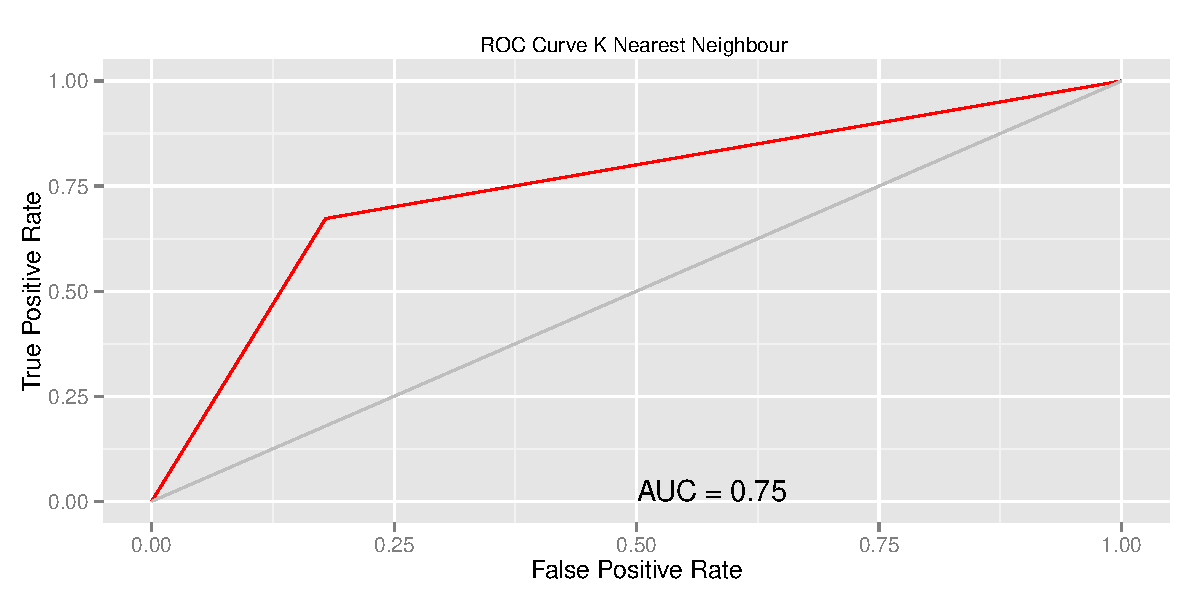
\includegraphics[width=\maxwidth]{figure/unnamed-chunk-101-1} \caption[ROC Curve - K Nearest Neighbour]{ROC Curve - K Nearest Neighbour}\label{fig:unnamed-chunk-101}
\end{figure}


\end{knitrout}
The Proportion of correct classification is:

\begin{knitrout}
\definecolor{shadecolor}{rgb}{0.969, 0.969, 0.969}\color{fgcolor}\begin{kframe}
\begin{alltt}
\hlstd{pcorrn3}\hlkwb{=}\hlnum{100}\hlopt{*}\hlkwd{sum}\hlstd{(ynew}\hlopt{==}\hlstd{nearest3)}\hlopt{/}\hlnum{100}
\hlstd{pcorrn3}
\end{alltt}
\begin{verbatim}
## [1] 157
\end{verbatim}
\end{kframe}
\end{knitrout}
We are applying Leave one out cross validation method here and the average accuracy obtained is 80.91\%:
\begin{knitrout}
\definecolor{shadecolor}{rgb}{0.969, 0.969, 0.969}\color{fgcolor}\begin{kframe}
\begin{alltt}
\hlstd{psum}\hlkwb{<-} \hlnum{0}
\hlstd{pcorr}\hlkwb{=}\hlkwd{dim}\hlstd{(}\hlnum{15}\hlstd{)}
\hlkwa{for} \hlstd{(k} \hlkwa{in} \hlnum{1}\hlopt{:}\hlnum{15}\hlstd{) \{}
  \hlstd{pred}\hlkwb{=}\hlkwd{knn.cv}\hlstd{(dataset,}\hlkwc{cl}\hlstd{=dataset}\hlopt{$}\hlstd{R01_credibility,k)}
  \hlstd{pcorr[k]}\hlkwb{=}\hlnum{100}\hlopt{*}\hlkwd{sum}\hlstd{(dataset}\hlopt{$}\hlstd{R01_credibility}\hlopt{==}\hlstd{pred)}\hlopt{/}\hlnum{1000}
  \hlstd{psum}\hlkwb{<-} \hlstd{psum}\hlopt{+}\hlstd{pcorr[k]}
\hlstd{\}}
\hlstd{pcorr}
\end{alltt}
\begin{verbatim}
##  [1] 76.6 77.4 80.3 79.0 82.0 81.4 82.4 82.1 82.6 82.0 81.8 81.2 81.2 81.3
## [15] 82.3
\end{verbatim}
\begin{alltt}
\hlstd{psum}\hlopt{/}\hlnum{15}
\end{alltt}
\begin{verbatim}
## [1] 80.90667
\end{verbatim}
\end{kframe}
\end{knitrout}
Thus all the above mentioned measures help to analyse the model well, and it was giving an accuracy of 78 \%, with specificity proportion of 0.67 and sensitivity of 0.82.\\
10 fold cross validation also applied in this model, each sub-sample's sensitivity ,specificity and accuracy is computed:
\begin{knitrout}
\definecolor{shadecolor}{rgb}{0.969, 0.969, 0.969}\color{fgcolor}\begin{kframe}
\begin{verbatim}
##   1   2   3   4   5   6   7   8   9  10 
## 100 100 100 100 100 100 100 100 100 100
##                  [,1]
## sensitivity 0.9722222
## sensitivity 0.9850746
## sensitivity 0.9027778
## sensitivity 0.9594595
## sensitivity 0.9859155
## sensitivity 0.9552239
## sensitivity 0.9545455
## sensitivity 0.9696970
## sensitivity 0.9358974
## sensitivity 0.9850746
##                  [,1]
## specificity 0.4285714
## specificity 0.5757576
## specificity 0.6071429
## specificity 0.3076923
## specificity 0.6206897
## specificity 0.4848485
## specificity 0.5882353
## specificity 0.5882353
## specificity 0.2272727
## specificity 0.5151515
##      [,1]
## acc1 0.82
## acc1 0.85
## acc1 0.82
## acc1 0.79
## acc1 0.88
## acc1 0.80
## acc1 0.83
## acc1 0.84
## acc1 0.78
## acc1 0.83
\end{verbatim}
\end{kframe}
\end{knitrout}
The average sensitivity is:
\begin{knitrout}
\definecolor{shadecolor}{rgb}{0.969, 0.969, 0.969}\color{fgcolor}\begin{kframe}
\begin{alltt}
\hlstd{sens.cv}\hlkwb{<-}\hlkwd{mean}\hlstd{(all.sense)}
\hlkwd{print}\hlstd{(sens.cv)}
\end{alltt}
\begin{verbatim}
## [1] 0.9605888
\end{verbatim}
\end{kframe}
\end{knitrout}
The average specificity is :
\begin{knitrout}
\definecolor{shadecolor}{rgb}{0.969, 0.969, 0.969}\color{fgcolor}\begin{kframe}
\begin{alltt}
\hlstd{spec.cv}\hlkwb{<-}\hlkwd{mean}\hlstd{(all.spese)}
\hlkwd{print}\hlstd{(spec.cv)}
\end{alltt}
\begin{verbatim}
## [1] 0.4943597
\end{verbatim}
\end{kframe}
\end{knitrout}
And the average accuracy using 10 fold cross validation is :
\begin{knitrout}
\definecolor{shadecolor}{rgb}{0.969, 0.969, 0.969}\color{fgcolor}\begin{kframe}
\begin{alltt}
\hlstd{acc1.cv}\hlkwb{<-}\hlkwd{mean}\hlstd{(all.acc1)}
\hlkwd{print}\hlstd{(acc1.cv)}
\end{alltt}
\begin{verbatim}
## [1] 0.824
\end{verbatim}
\end{kframe}
\end{knitrout}

\subsection{Random Forest}\hspace{0.9cm} A random forest is an ensemble (i.e., a collection) of un-pruned
decision trees. Ensemble models are often robust to variance and bias. Random forests are often used when we have large training datasets and particularly a very large number of input variables (hundreds or even
thousands of input variables). The algorithm is efficient with respect to a large number of variables since it repeatedly subsets the variables available. We can make use of this model to view the relative importance of each variable also. A random forest model is typically made up of tens or hundreds of decision trees \cite{[5]}.\par

The \textit{randomForest} package provides the 'randomForest' function. The code snippet building random forest model is given below:

\begin{knitrout}
\definecolor{shadecolor}{rgb}{0.969, 0.969, 0.969}\color{fgcolor}\begin{kframe}
\begin{alltt}
\hlkwd{library}\hlstd{(randomForest,} \hlkwc{quietly}\hlstd{=}\hlnum{TRUE}\hlstd{)}
\hlkwd{set.seed}\hlstd{(crv}\hlopt{$}\hlstd{seed)}
\hlstd{rf} \hlkwb{<-} \hlstd{randomForest}\hlopt{::}\hlkwd{randomForest}\hlstd{(}\hlkwd{as.factor}\hlstd{(R01_credibility)} \hlopt{~} \hlstd{.,}
                                 \hlkwc{data}\hlstd{=dataset[sample,}\hlkwd{c}\hlstd{(input, target)],}
                                 \hlkwc{ntree}\hlstd{=}\hlnum{500}\hlstd{,}
                                 \hlkwc{mtry}\hlstd{=}\hlnum{4}\hlstd{,}
                                 \hlkwc{importance}\hlstd{=}\hlnum{TRUE}\hlstd{,}
                                 \hlkwc{na.action}\hlstd{=randomForest}\hlopt{::}\hlstd{na.roughfix,}
                                 \hlkwc{replace}\hlstd{=}\hlnum{FALSE}\hlstd{)}
\end{alltt}
\end{kframe}
\end{knitrout}
The textual output of random forest model is:
\begin{knitrout}
\definecolor{shadecolor}{rgb}{0.969, 0.969, 0.969}\color{fgcolor}\begin{kframe}
\begin{alltt}
\hlkwd{print}\hlstd{(rf)}
\end{alltt}
\begin{verbatim}
## 
## Call:
##  randomForest(formula = as.factor(R01_credibility) ~ ., data = dataset[sample,      c(input, target)], ntree = 500, mtry = 4, importance = TRUE,      replace = FALSE, na.action = randomForest::na.roughfix) 
##                Type of random forest: classification
##                      Number of trees: 500
## No. of variables tried at each split: 4
## 
##         OOB estimate of  error rate: 24.12%
## Confusion matrix:
##     0   1 class.error
## 0 494  61   0.1099099
## 1 132 113   0.5387755
\end{verbatim}
\end{kframe}
\end{knitrout}
The \textit{pROC} package implements various AUC functions.
\begin{knitrout}
\definecolor{shadecolor}{rgb}{0.969, 0.969, 0.969}\color{fgcolor}\begin{kframe}
\begin{alltt}
\hlcom{# Calculate the Area Under the Curve (AUC).}

\hlstd{pROC}\hlopt{::}\hlkwd{roc}\hlstd{(rf}\hlopt{$}\hlstd{y,} \hlkwd{as.numeric}\hlstd{(rf}\hlopt{$}\hlstd{predicted))}
\end{alltt}
\begin{verbatim}
## 
## Call:
## roc.default(response = rf$y, predictor = as.numeric(rf$predicted))
## 
## Data: as.numeric(rf$predicted) in 555 controls (rf$y 0) < 245 cases (rf$y 1).
## Area under the curve: 0.6757
\end{verbatim}
\begin{alltt}
\hlcom{# Calculate the AUC Confidence Interval.}

\hlstd{pROC}\hlopt{::}\hlkwd{ci.auc}\hlstd{(rf}\hlopt{$}\hlstd{y,} \hlkwd{as.numeric}\hlstd{(rf}\hlopt{$}\hlstd{predicted))}
\end{alltt}
\begin{verbatim}
## 95% CI: 0.6418-0.7095 (DeLong)
\end{verbatim}
\end{kframe}
\end{knitrout}
From this model we will get the importance of variables:
\begin{knitrout}
\definecolor{shadecolor}{rgb}{0.969, 0.969, 0.969}\color{fgcolor}\begin{kframe}
\begin{alltt}
\hlstd{rn} \hlkwb{<-} \hlkwd{round}\hlstd{(randomForest}\hlopt{::}\hlkwd{importance}\hlstd{(rf),} \hlnum{2}\hlstd{)}
\hlstd{rn[}\hlkwd{order}\hlstd{(rn[,}\hlnum{3}\hlstd{],} \hlkwc{decreasing}\hlstd{=}\hlnum{TRUE}\hlstd{),]}
\end{alltt}
\begin{verbatim}
##                      0     1 MeanDecreaseAccuracy MeanDecreaseGini
## TNM_check_status 17.94 33.19                31.84            25.38
## duration         17.04  7.83                19.05            22.11
## TNM_history      10.94 11.81                15.44            14.53
## credit           12.64  3.34                12.72            29.98
## TNM_guarantor    12.03  3.45                11.65             4.40
## TNM_bonds         0.66 10.54                 6.56             9.96
## TNM_purpose       4.86  2.92                 5.74            14.58
## TNM_install       6.68 -0.03                 5.64             6.68
## TNM_property      8.34 -2.28                 5.52            10.16
## age               4.60  2.55                 5.31            23.18
## nocredit          4.33 -0.64                 3.25             4.59
## TNM_ph            2.39  2.21                 3.17             4.57
## TNM_nri           1.86  2.31                 2.84             1.10
## TNM_jobex         1.10  3.06                 2.77            11.22
## TNM_s_status      1.24  2.84                 2.77             8.48
## TNM_job           3.12 -0.32                 2.49             7.36
## rate              2.73 -0.33                 2.00             9.32
## TNM_house         3.41 -2.36                 1.55             5.48
\end{verbatim}
\end{kframe}
\end{knitrout}
Random Forest gives less importance to the ignored variables \textit{liable} and \textit{residance} by running in original dataset, which makes the assumption made in preprocessing part strong. Figure [11] shows the relative importance of the variables:
\begin{knitrout}
\definecolor{shadecolor}{rgb}{0.969, 0.969, 0.969}\color{fgcolor}\begin{kframe}
\begin{alltt}
\hlstd{randomForest}\hlopt{::}\hlkwd{varImpPlot}\hlstd{(rf,} \hlkwc{main}\hlstd{=}\hlstr{""}\hlstd{)}
\hlkwd{title}\hlstd{(}\hlkwc{main}\hlstd{=}\hlstr{"Variable Importance Random Forest"}\hlstd{,}
      \hlkwc{sub}\hlstd{=}\hlkwd{paste}\hlstd{(}\hlstr{"Rattle"}\hlstd{,} \hlkwd{format}\hlstd{(}\hlkwd{Sys.time}\hlstd{(),} \hlstr{"%Y-%b-%d %H:%M:%S"}\hlstd{),} \hlkwd{Sys.info}\hlstd{()[}\hlstr{"user"}\hlstd{]))}
\end{alltt}
\end{kframe}\begin{figure}
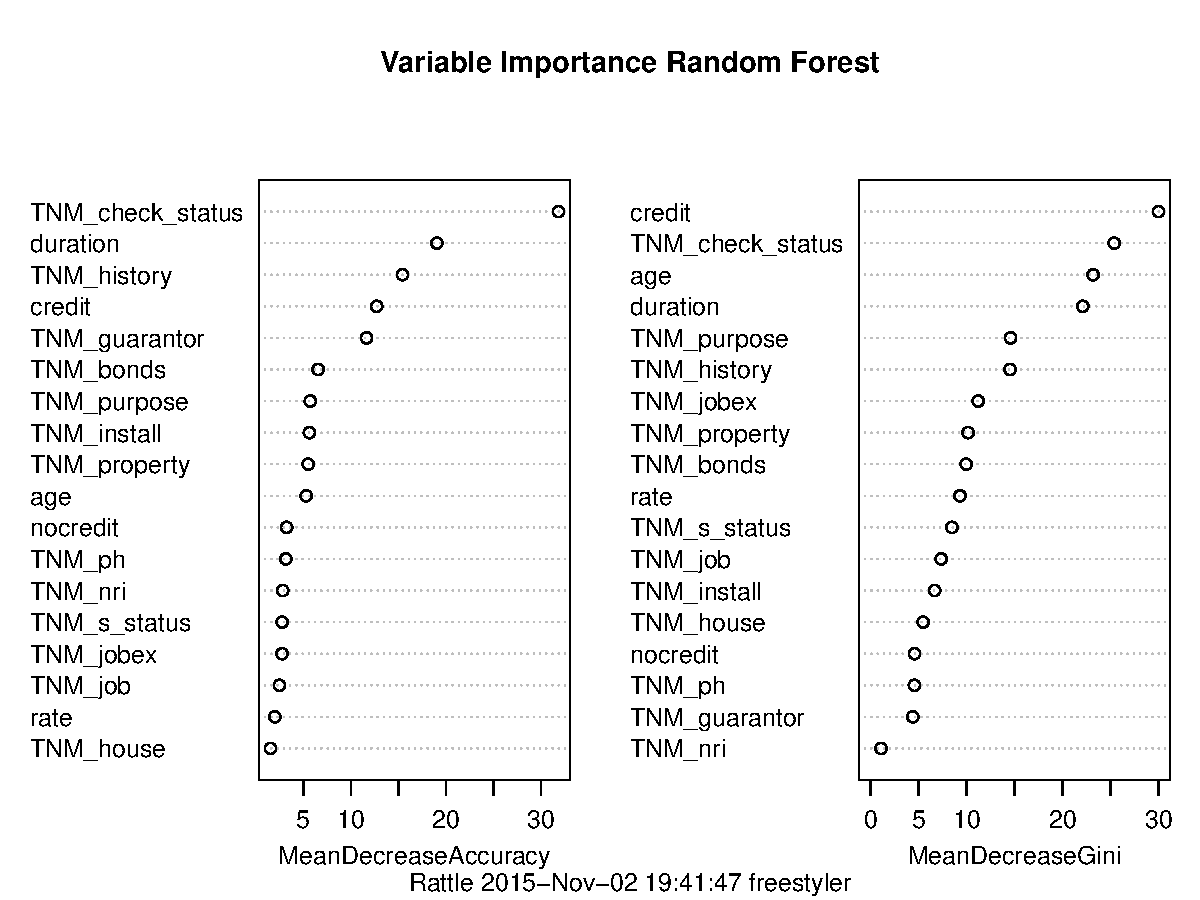
\includegraphics[width=\maxwidth]{figure/unnamed-chunk-114-1} \caption[Random Forest - Variable Importance]{Random Forest - Variable Importance}\label{fig:unnamed-chunk-114}
\end{figure}


\end{knitrout}
\hspace{0.5cm} Gini importance \cite{[6]} : The variable importance metric refers to the Gini used for asserting model performance which is not closely related to AUC. Every time a split of a node is made on variable m the gini impurity criterion for the two descendent nodes is less than the parent node. Adding up the gini decreases for each individual variable over all trees in the forest gives a fast variable importance that is often very consistent with the permutation importance measure.\\
Each tree can be displayed using below script ,where 1 is the tree number :
\begin{knitrout}
\definecolor{shadecolor}{rgb}{0.969, 0.969, 0.969}\color{fgcolor}\begin{kframe}
\begin{alltt}
\hlkwd{printRandomForests}\hlstd{(rf,} \hlnum{1}\hlstd{)}
\end{alltt}
\end{kframe}
\end{knitrout}
An ROC (receiver operator characteristic) curve shown in Figure [12] compares the false positive rate to the true positive rate. We can access the trade off the number of observations that are incorrectly classified as positives against the number of observations that are correctly classified as positives.

\begin{knitrout}
\definecolor{shadecolor}{rgb}{0.969, 0.969, 0.969}\color{fgcolor}\begin{kframe}
\begin{alltt}
\hlkwd{print}\hlstd{(p)}
\end{alltt}
\end{kframe}\begin{figure}
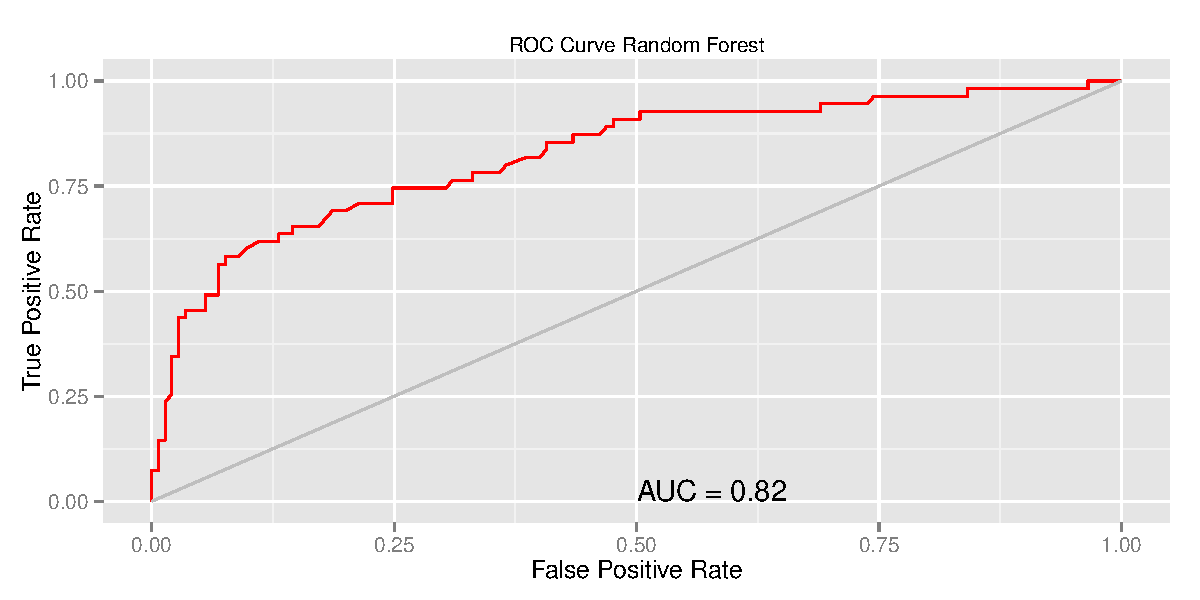
\includegraphics[width=\maxwidth]{figure/unnamed-chunk-117-1} \caption[Random Forest - ROC Curve]{Random Forest - ROC Curve}\label{fig:unnamed-chunk-117}
\end{figure}


\end{knitrout}
The confusion matrix showing counts and proportions shown below:
\begin{knitrout}
\definecolor{shadecolor}{rgb}{0.969, 0.969, 0.969}\color{fgcolor}\begin{kframe}
\begin{alltt}
\hlstd{pr} \hlkwb{<-} \hlkwd{predict}\hlstd{(rf,} \hlkwc{newdata}\hlstd{=}\hlkwd{na.omit}\hlstd{(dataset[test,} \hlkwd{c}\hlstd{(input, target)]))}

\hlkwd{table}\hlstd{(}\hlkwd{na.omit}\hlstd{(dataset[test,} \hlkwd{c}\hlstd{(input, target)])}\hlopt{$}\hlstd{R01_credibility, pr,}
      \hlkwc{dnn}\hlstd{=}\hlkwd{c}\hlstd{(}\hlstr{"Actual"}\hlstd{,} \hlstr{"Predicted"}\hlstd{))}
\end{alltt}
\begin{verbatim}
##       Predicted
## Actual   0   1
##      0 137   8
##      1  28  27
\end{verbatim}
\end{kframe}
\end{knitrout}


\begin{knitrout}
\definecolor{shadecolor}{rgb}{0.969, 0.969, 0.969}\color{fgcolor}\begin{kframe}
\begin{alltt}
\hlkwd{pcme}\hlstd{(}\hlkwd{na.omit}\hlstd{(dataset[test,} \hlkwd{c}\hlstd{(input, target)])}\hlopt{$}\hlstd{R01_credibility, pr)}
\end{alltt}
\begin{verbatim}
##       Predicted
## Actual    0    1 Error
##      0 0.68 0.04  0.06
##      1 0.14 0.14  0.51
\end{verbatim}
\end{kframe}
\end{knitrout}
From the above computations, this model can also be used to analyse the variable importance. Random Forest gives an accuracy of 82\%, but specificity proportion 0.49 only.\\
The 10 fold cross validation computation as follows:
\begin{knitrout}
\definecolor{shadecolor}{rgb}{0.969, 0.969, 0.969}\color{fgcolor}\begin{kframe}
\begin{verbatim}
##   1   2   3   4   5   6   7   8   9  10 
## 100 100 100 100 100 100 100 100 100 100
\end{verbatim}
\end{kframe}
\end{knitrout}
Each sub-sample's of sensitivity ,specificity and error rate:
\begin{knitrout}
\definecolor{shadecolor}{rgb}{0.969, 0.969, 0.969}\color{fgcolor}\begin{kframe}
\begin{verbatim}
##                  [,1]
## sensitivity 0.9166667
## sensitivity 0.9104478
## sensitivity 0.9027778
## sensitivity 0.9189189
## sensitivity 0.9577465
## sensitivity 0.9402985
## sensitivity 0.9090909
## sensitivity 0.8939394
## sensitivity 0.8974359
## sensitivity 0.9104478
##                  [,1]
## specificity 0.5000000
## specificity 0.4545455
## specificity 0.5000000
## specificity 0.3076923
## specificity 0.4482759
## specificity 0.3939394
## specificity 0.3823529
## specificity 0.4117647
## specificity 0.3181818
## specificity 0.4242424
##      [,1]
## acc1 0.80
## acc1 0.76
## acc1 0.79
## acc1 0.76
## acc1 0.81
## acc1 0.76
## acc1 0.73
## acc1 0.73
## acc1 0.77
## acc1 0.75
\end{verbatim}
\end{kframe}
\end{knitrout}
Because we have the same number of examples in each fold, we can compute unweighted mean. This is the average of sub-sample's sensitivity:
\begin{knitrout}
\definecolor{shadecolor}{rgb}{0.969, 0.969, 0.969}\color{fgcolor}\begin{kframe}
\begin{verbatim}
## [1] 0.915777
\end{verbatim}
\end{kframe}
\end{knitrout}
This is the average of sub-sample's specificity:
\begin{knitrout}
\definecolor{shadecolor}{rgb}{0.969, 0.969, 0.969}\color{fgcolor}\begin{kframe}
\begin{verbatim}
## [1] 0.4140995
\end{verbatim}
\end{kframe}
\end{knitrout}
This is the cross validation average accuracy proportion:
\begin{knitrout}
\definecolor{shadecolor}{rgb}{0.969, 0.969, 0.969}\color{fgcolor}\begin{kframe}
\begin{verbatim}
## [1] 0.766
\end{verbatim}
\end{kframe}
\end{knitrout}

\section{Result and Discussions}\hspace{0.9cm}In this section we are discussing about the results we found from exploratory data analysis onwards to each model's evaluation stage. \par
\hspace{0.5cm} In data analysis stage we conducted chi squared statistics to categorical data but could not reach any conclusion that impact on the independent variable. In t-statistics p value of two varailbes named "liable", and "residence" were varying drastically hence we assumed that it could not contribute well in output prediction. In addition to that using random forest the obtained variable significance plot also shows those two variables as less significant ones'. The principal componenet analysis was done, and 18 components were giving above 95 percent of the variance. Hence we made PCA Neural network model and analysed its performance as mentioned in section 6.4.1. \par
\hspace{0.5cm} The ROC graph is a technique for visualizing, organizing and selecting classifiers based on their performance. Comparison of two or more ROC curves is usually based on a comparison of the area measures. The ROC curves of all models is shown in Figure[13] and their area under curve value is showin Table[3]. \par
\begin{figure}[h]
\begin{center}
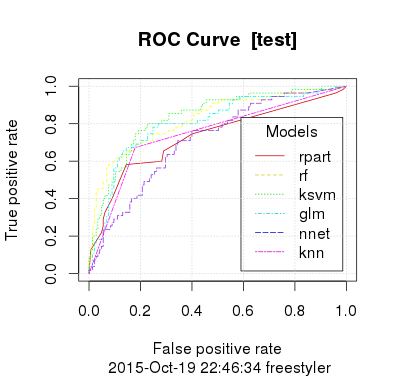
\includegraphics [scale=0.80]{ROc.png}
\end{center}
\caption{ROC Curve comparison of models}
\end{figure}

\begin{table}[t]
\caption{Comparison of models}
\centering
\begin{tabular}{c|c|c}
\toprule
Model No & Model & Area Under Curve \\
\midrule
1 & Logistic Regression & 0.8 \\
2 & Decision Tree & 0.73 \\
3 & Support Vector Machine & 0.82 \\
4 & Neural Networks & 0.71 \\
5 & K Nearest Neighbour & 0.75 \\
6 & Random Forest & 0.82 \\

\bottomrule
\end{tabular}
\label{tab}
\end{table}
Table[4] shows each model's sensitivity, specificity and accuracy without 10 fold cross validation and Table[5] with 10 fold cross validation.
\begin{table}[t]
\caption{Performance measures}
\centering
\begin{tabular}{c|c|c|c|c}
\toprule
Model No & Model & Sensitivity & Specificity & Accuracy \\
\midrule
1 & Logistic Regression & 0.9 & 0.51 & 0.795\\
2 & Decision Tree & 0.86 & 0.58 & 0.78\\
3 & Support Vector Machine & 0.90 & 0.50 & 0.795 \\
4 & Neural Networks & 0.76 & 0.51 & 0.69\\
5 & K Nearest Neighbour & 0.82 & 0.673 & 0.78\\
6 & Random Forest & 0.945 & 0.491 & 0.82\\
\bottomrule
\end{tabular}
\label{tab}
\end{table}

\begin{table}[t]
\caption{Performance of measures with 10 FCV}
\centering
\begin{tabular}{c|c|c|c|c}
\toprule
Model No & Model & Sensitivity & Specificity & Accuracy \\
\midrule
1 & Logistic Regression & 0.88 & 0.46 & 0.76\\
2 & Decision Tree & 0.88 & 0.37 & 0.73\\
3 & Support Vector Machine & 0.90 & 0.42 & 0.76 \\
4 & Neural Networks & 0.79 & 0.45 & 0.69\\
5 & K Nearest Neighbour & 0.96 & 0.49 & 0.82\\
6 & Random Forest & 0.91 & 0.41 & 0.77\\
\bottomrule
\end{tabular}
\label{tab}
\end{table}


%\subsection{Including tables}
%Include some summary tables of the data as as shown in table \ref{summary-data}. Make sure you discuss about the table you have included and explain the facts it is revealing. You have to sell your table in a way that the reader will understand that this table was awesome and it reveals a fact the reader would otherwise not recognize.\\

%Notice that we used the function \texttt{xtable()} form the \textbf{R} package \texttt{xtable} \cite{xtab} to generate a pretty table. \texttt{knitr} does this using \LaTeX{} codes generated by \texttt{xtable} and automatically put it in a nicer we and we don't have to worry about its position. Also notice how we write the caption of the table as well as refer the table \ref{summary-data} from the text.

%\subsection{Including figures} Please don't forget to add nice data plots in your documents. Plots are nice to conveying message and much better than tables. Discuss what facts the figure is revealing and refer the figure from the text as figure \ref{fig:data-plot}.
%
%<<data-plot, fig.width=5, fig.height=5, fig.align='center', fig.cap="Awesome figure caption" ,out.width='.6\\linewidth',fig.pos="hbtp">>=
%plot(trees)
%@


\section{Conclusion} \hspace{0.9cm}This report illustrated the study of classification task in german credit dataset. Varoius data mining techniques applied to the dataset, after pre processing techniques. Each model analysed with its performance measures. In section 7 all the models compared with and without 10 fold cross validation as well with ROC curves. Based on the Area Under curve measure from Table[3] we can say that Logistic regression, Support Vector Machine and Random Forest have almost near AUC value and are better than other models.\par
\hspace{0.5cm}The dataset information, \cite{[2]} mentioned "It is worse to class a customer as good when they are bad (5), than it is to class a customer as bad when they are good (1)". Based on that while analysing the specificity of each model with out 10 FCV, k nearest neighbour giving more value, but among Logistic regression, Support Vector Machine and Random Forest, Logistic Regression has more specificity value with and without 10 FCV.\par
\hspace{0.5cm}Based on ROC and accuracy Random Forest model performed well. We can ignore the models Neural network and Decision Tree based on their poor performance compared to other models.
%The conclusion is an elaboration of your abstract. Here you will discuss what you have done and how. The gist of the results need to be mentioned here. It needs to be convincing and the reader will never regret forgetting the date. Please keep it in mind that there may be readers who only read your conclusion. So, make your conclusion complete so that no reader misses anything even if they don't want to read the whole document.\\

%Each paragraph of the conclusion may discuss one result you have found or one concept you are proposing. Discuss your findings and why it is better and how it is compared to any existing methods may exist. \\

%Please don't forget to cite the works of others if you used it in your analysis. The citation is important for two reasons. Fist of all it acknowledges the good works other people have done which encourages them keep continue doing their good work. Second, it protects you from plagiarism which is a very nasty task everyone should avoid.\\

%There should be one paragraph about the future direction of the work you have done. You would like to make it so fascinating that the reader would wish to be involved in this work in future. \\

%Finally this is just a template. Your exact document may have a very different outlook. It demonstrates how you can start to write a document. Our biggest problem is to figure out where to start from. And this documents provides a guide for that. I hope it turns out to be helpful for some of the readers. If you have any comments or concern about this document please let me know so that I can improve this document. 

\newpage

\begin{thebibliography}{9}

\bibitem{ubover}
    Andrea Dal Pozzolo, Olivier Caelen and Gianluca Bontempi,
    \emph{unbalanced: Racing for Unbalanced Methods Selection},
    R package version 2.0,
    http://cran.r-project.org/web/packages/unbalanced, 
    2015

\bibitem{dataset}
  M. Lichman , \emph{{UCI} Machine Learning Repository}.
  University of California, Irvine, School of Information and Computer Sciences
  http://archive.ics.uci.edu/ml
  2013.
  
\bibitem{IDRE}
  Institute for Digital Research and Education
  \emph{What statistical analysis should I use},
  UCLA:Statistical Consulting Group.  
  http://www.ats.ucla.edu/stat/mult\_pkg/whatstat/., 
  (accessed October 07, 2015)  

\bibitem{BDA}
  Johannes Ledolter, \emph{DATA MINING AND BUSINESS ANALYTICS WITH R},
  Department of Management Sciences, Tippie College of Business,
  University of Iowa.
  2013.

\bibitem{rattle}
    Graham J Williams,
    \emph{Rattle: A Data Mining GUI for R},
    The R Journal,Vol 1,Pages 45-55
    http://journal.r-project.org/archive/2009-2/RJournal\_2009-2\_Williams.pdf,
    Dec, 2009.

\bibitem{rf}
    Leo Breiman, Adele Cutler and Andy Liaw, Matthew Wiener,
    \emph{Breiman and Cutler's Random Forests for Classification and Regression},
    Version 4.6-12, Repository CRAN,
    http://www.stat.berkeley.edu/~breiman/RandomForests/, 
    2015.

\bibitem{nnet}
    Brian Ripley ,William Venables,
    \emph{Feed-Forward Neural Networks and Multinomial Log-Linear Models},
    Package nnet,Version 7.3-11, Repository CRAN,
    https://cran.r-project.org/web/packages/nnet/, 
    2015.

\bibitem{nnet}
    Brian Ripley ,William Venables,
    \emph{Neural Networks with a Principal Component Step },
    Package caret, Version: 6.0-24,
    http://www.inside-r.org/packages/cran/caret/docs/pcaNNet.default, 
    (accessed October 31, 2015).

\end{thebibliography}

\newpage
\begin{flushleft}
{\Large\textbf{Appendix}}\\\\
\end{flushleft}

\textbf{Attribute Information:}\\
Attribute 1: (qualitative)\\
\textbf{Renamed as \textit{$TNM\_ check\_ status$}\\
Recoded to numeric values [1,2,3,4] respectively.}\\
Status of existing checking account\\
A11 : ... $\< $0 DM\\
A12 : 0 $\leq$ ... $\<$ 200 DM\\
A13 : ... $\geq$ 200 DM / salary assignments for at least 1 year\\
A14 : no checking account\\
\\
Attribute 2: (numerical)\\
Duration in month\\
\\
Attribute 3: (qualitative) \\
\textbf{Renamed as \textit{$TNM\_ history$}}\\
\textbf{Recoded to numeric values [1,2,3,4,5] respectively.}\\
Credit history\\
A30 : no credits taken/ all credits paid back duly\\
A31 : all credits at this bank paid back duly\\
A32 : existing credits paid back duly till now\\
A33 : delay in paying off in the past\\
A34 : critical account/ other credits existing (not at this bank)\\
\\
Attribute 4: (qualitative)\\
\textbf{Renamed as \textit{$TNM\_ purpose$}}\\
\textbf{Recoded to numeric values [1 to 11] respectively.}\\
Purpose\\
A40 : car (new)\\
A41 : car (used)\\
A42 : furniture/equipment\\
A43 : radio/television\\
A44 : domestic appliances\\
A45 : repairs\\
A46 : education\\
A47 : (vacation - does not exist\?)\\
A48 : retraining\\
A49 : business\\
A410 : others\\
\\
Attribute 5: (numerical)\\
Credit amount\\
\\
Attibute 6: (qualitative)\\
\textbf{Renamed as \textit{$TNM\_ bonds$}}\\
\textbf{Recoded to numeric values [1 to 5] respectively.}\\
Savings account/bonds\\
A61 : ... $\<$ 100 DM
A62 : 100 $\leq$ ... $\<$ 500 DM\\
A63 : 500 $\leq$ ... $\<$ 1000 DM\\
A64 : .. $\geq$ 1000 DM\\
A65 : unknown/ no savings account\\
\\
Attribute 7: (qualitative)\\
\textbf{Renamed as \textit{$TNM\_ jobex$}}\\
\textbf{Recoded to numeric values [1 to 5] respectively.}\\
Present employment since\\
A71 : unemployed\\
A72 : ... $\<$ 1 year\\
A73 : 1 $\leq$ ... $\<$ 4 years\\
A74 : 4 $\leq$ ... $\<$ 7 years\\
A75 : .. $\geq$ 7 years\\
\\
Attribute 8: (numerical)\\
Installment rate in percentage of disposable income\\
\\
Attribute 9: (qualitative)\\
\textbf{Renamed as \textit{$TNM\_ s\_ status$}}\\
\textbf{Recoded to numeric values [1 to 5] respectively.}\\
Personal status and sex\\
A91 : male : divorced/separated\\
A92 : female : divorced/separated/married\\
A93 : male : single\\
A94 : male : married/widowed\\
A95 : female : single\\
\\
Attribute 10: (qualitative)\\
\textbf{Renamed as \textit{$TNM\_ guarantor$}}\\
\textbf{Recoded to numeric values [1 to 3] respectively.}\\
Other debtors / guarantors\\
A101 : none\\
A102 : co-applicant\\
A103 : guarantor\\
\\
Attribute 11: (numerical)\\
Present residence since\\
\\
Attribute 12: (qualitative)\\
\textbf{Renamed as \textit{$TNM\_ property$}}\\
\textbf{Recoded to numeric values [1 to 4] respectively.}\\
Property\\
A121 : real estate\\
A122 : if not A121 : building society savings agreement/ life insurance\\
A123 : if not A121/A122 : car or other, not in attribute 6\\
A124 : unknown / no property\\
\\
Attribute 13: (numerical)\\
Age in years\\
\\
Attribute 14: (qualitative)\\
\textbf{Renamed as \textit{$TNM\_ install$}}\\
\textbf{Recoded to numeric values [1 to 3] respectively.}\\
Other installment plans\\
A141 : bank\\
A142 : stores\\
A143 : none\\
\\
Attribute 15: (qualitative)\\
\textbf{Renamed as \textit{$TNM\_ house$}}\\
\textbf{Recoded to numeric values [1 to 3] respectively.}\\
Housing\\
A151 : rent\\
A152 : own\\
A153 : for free\\
\\
Attribute 16: (numerical)\\
Number of existing credits at this bank\\
\\
Attribute 17: (qualitative)\\
\textbf{Renamed as \textit{$TNM\_ job$}}\\
\textbf{Recoded to numeric values [1 to 4] respectively.}\\
Job\\
A171 : unemployed/ unskilled - non-resident\\
A172 : unskilled - resident\\
A173 : skilled employee / official\\
A174 : management/ self-employed/\\
highly qualified employee/ officer\\
\\
Attribute 18: (numerical)\\
Number of people being liable to provide maintenance for\\
\\
Attribute 19: (qualitative)\\
\textbf{Renamed as \textit{$TNM\_ ph$}}\\
\textbf{Recoded to numeric values [1 - 2] respectively.}\\
Telephone\\
A191 : none\\
A192 : yes, registered under the customers name\\
\\
Attribute 20: (qualitative)\\
\textbf{Renamed as \textit{$TNM\_ nri$}}\\
\textbf{Recoded to numeric values [1 -2] respectively.}\\
foreign worker\\
A201 : yes\\
A202 : no \\
\\
Attribute 21: (Target variable)\\
\textbf{Renamed as \textit{$R01\_ credibility$}}\\
\textbf{Recoded to numeric values [0-1] respectively.}\\
Labels\\
0 : Good\\
1 : Bad \\

\end{document}
